\documentclass[usenames,dvipsnames]{beamer}

%%%%%%%%%%%%%%%%%%%%%%%%%%%%%%%%%%%%%%%%%%%%%
% PACKAGES
%%%%%%%%%%%%%%%%%%%%%%%%%%%%%%%%%%%%%%%%%%%%%

% STANDARD

\usepackage{etoolbox}
\usepackage{xparse}
\usepackage{graphicx}
\usepackage{subcaption}
\usepackage{float}
\usepackage{xstring}
\usepackage{diagbox}
\usepackage{changepage} % https://tex.stackexchange.com/a/160827/145331

% PROOF READING

\usepackage[utf8]{inputenc}
\usepackage[english]{babel}

% TIKZ

\usepackage{tikz}
\usetikzlibrary{arrows.meta, matrix, arrows,automata,positioning}

% FONTS AND COLORS

\usepackage{xcolor}
\usepackage{cancel}
\usepackage{anyfontsize}
\usepackage{moresize}
\usepackage{bm} %use bold in math

% TABLES

\usepackage{makecell} % https://tex.stackexchange.com/a/11694/145331
\usepackage{multirow}

% THEOREMS & MATHS

\usepackage{amsmath}
\usepackage{amsthm}
\usepackage{amssymb}
\usepackage{mathtools}
\usepackage{calc}

% ALGORITHMS

\usepackage[ruled,vlined,linesnumbered]{algorithm2e}

%%%%%%%%%%%%%%%%%%%%%%%%%%%%%%%%%%%%%%%%%%%%%
% IMPORTS OF CUSTOM COMMANDS
%%%%%%%%%%%%%%%%%%%%%%%%%%%%%%%%%%%%%%%%%%%%%

\usepackage{calculator}

%%%%%%%%%%%%%%%%%%%%%%%%%%%%%%%%%%%%%%%%%%%%%
% REFERENCES
%%%%%%%%%%%%%%%%%%%%%%%%%%%%%%%%%%%%%%%%%%%%%

\makeatletter

\NewDocumentCommand{\appendixref}{m}{%
    Appendix \ref{#1}%
}

% Add a reference to a equation
% param1 the label of the equation
\NewDocumentCommand{\equationref}{m}{%
    Equation \eqref{#1}%
}

% Add a reference to a algorithm line
% param1 the label of the algorithm line
\NewDocumentCommand{\lineref}{m}{%
    Line \ref{#1}%
}

% Add a reference to a algorithm line
% param1 the label of the algorithm where piece starts
% param1 the label of the algorithm where priece ends
\NewDocumentCommand{\linesref}{m m}{%
    Lines \ref{#1}--\ref{#2}%
}

% Add a reference to an algorithm
% param1 the label of the algorithm
\NewDocumentCommand{\algref}{m}{%
    Algorithm \ref{#1}%
}

% Add a reference to a definition
% param1 the label of the definition
\NewDocumentCommand{\defref}{m}{%
    Definition \ref{#1}%
}

% Add a reference to a definition
% param1 the label of the first definition
% param2 the label of the second definition
\NewDocumentCommand{\defsref}{m m}{%
    Definitions \ref{#1}--\ref{#2}%
}

% Add a reference to a figure
% param1 the label of the figure
\NewDocumentCommand{\figref}{m}{%
    Figure \ref{#1}%
}

% Add a reference to a range of figure
% param1 the label of the first figure in the range (inclusive)
% param2 the label of the last figure in the range (inclusive)
\NewDocumentCommand{\figsref}{m m}{%
    Figures \ref{#1}--\ref{#2}%
}


\NewDocumentCommand{\r@figrefs}{m}{%
    \@ifnextchar\bgroup{, \ref{#1}\r@figrefs}{ and \ref{#1}}%
}
% Add a reference to a figure
% param1 the label of the figure
\NewDocumentCommand{\figrefs}{m}{%
    Figures \ref{#1}\r@figrefs%
}

% Add a reference to a table
% param1 the label of the table
\NewDocumentCommand{\tblref}{m}{%
    Table \ref{#1}%
}

% Add a reference to a theorem
% param1 the label of the table
\NewDocumentCommand{\thmref}{m}{%
    Theorem \ref{#1}%
}

% Add a reference to a lemma
% param1 the label of the lemma
\NewDocumentCommand{\lemmaref}{m}{%
    Lemma \ref{#1}%
}

% Add a reference to an example
% param1 the label of the example
\NewDocumentCommand{\exampleref}{m}{%
    Example \ref{#1}%
}

%Add a reference to a section
% param1 the section to refer
\NewDocumentCommand{\secref}{m}{%
    Section \ref{#1}%
}

\NewDocumentCommand{\chapterref}{m}{%
    Chapter \ref{#1}%
}

%%%%%%%%%%%%%%%%%%%%%%%%%%%%%%%%%%%%%%%%%%%%%
% MATHS COMMANDS
%%%%%%%%%%%%%%%%%%%%%%%%%%%%%%%%%%%%%%%%%%%%%

% Print the ceil of a number
\NewDocumentCommand{\ceilOf}{m}{%
    \wrapMath{\lceil{#1}\rceil}%
}

% Print the floor of a number
\NewDocumentCommand{\floorOf}{m}{%
    \wrapMath{\lfloor{#1}\rfloor}%
}


%%%%%%%%%%%%%%%%%%%%%%%%%%%%%%%%%%%%%%%%%%%%%
% USEFUL COMMANDS
%%%%%%%%%%%%%%%%%%%%%%%%%%%%%%%%%%%%%%%%%%%%%

%DOES NOT WORK
\NewDocumentEnvironment{verticalAlign}{+b}{%
    \topskip0pt%
    \vspace*{\fill}%
    {#1}%
    \vspace*{\fill}%
}{%
}

% Indent a body of text
% param1 dimension representing the space you want to indent
% param2 body actual content to put in the indented wall of text
\NewDocumentEnvironment{indentText}{O{3cm} +b}{%
    \begin{minipage}{\dimexpr\textwidth-#1}%
        #2%
        \xdef\tpd{\the\prevdepth}%
    \end{minipage}%
}{%
}

% Put a definition block in the text
%
% param1 the definition name. If not specified we won't have a definition
% param2 the label we want this definition to have. Input of \label. If not specified we won't put the \label command
% param3 the content of the definition
% \NewDocumentEnvironment{definition}{o o +b}{%
%     %BEGIN
%     \IfNoValueTF{#1}{%
%         \begin{theorem}%
%     }{%
%         \begin{theorem}[#1]%
%     }%
%     \IfNoValueF{#2}{%
%         \label{#2}%
%     }%
%     #2%
%     \end{theorem}%
% }{%
%     %END
% }
%     \IfNoValueTF{#1}{%
%         \begin{theorem}
%     }{%
%     }%
% }

\NewDocumentCommand{\setFontSize}{m o m}{%
    \IfNoValueF{#2}{%
        \fontsize{#1}{#2}\selectfont#3%
    }{%
        % see https://texblog.org/2012/08/29/changing-the-font-size-in-latex/
        \MULTIPLY{#1}{1.2}{\setFont@baseline}%
        \fontsize{#1}{\setFont@baseline}\selectfont#3%
    }%
}

% Adds a todo embedded in the text (colored blue)
% param1: an optional star: if a star is present, we will put the todo as a footnote
% param2: the text to put
\NewDocumentCommand{\todo}{s m}{%
    % \IfBooleanTF{#1}{%
    %     \footnote{\color{blue} #2}%
    % }{%
    %     {\color{blue} #2}%
    % }%
}

% Mask a todo embedded in the text (colored blue). 
% param1: an optional star: if a star is present, we will put the todo as a footnote
% param2: the text to put
\NewDocumentCommand{\todook}{s m}{%
}

%Adds a todo as a footnoe
\NewDocumentCommand{\code}{m}{%
    \texttt{#1}%
}

% draw a square.
% param1: fill color red!50
% param2: border color (default to black)
\NewDocumentCommand{\drawFilledSquare}{m O{black}}{%
    \begin{tikzpicture}%
        \node [rectangle,draw={#2},fill={#1}] (m) at (0,0) {};%
    \end{tikzpicture}%
}

% print a computer science ordered pair
% param1 first element of the pair
% param2 second element of the pair
\NewDocumentCommand{\paircs}{m m}{%
    \wrapMath{\langle {#1}, {#2} \rangle }%
}

\NewDocumentEnvironment{coloredBlock}{m O{blue} O{white}}{%
\setbeamercolor{block title}{bg=#2, fg=#3}
    \begin{block}{#1}%
}{%
    \end{block}%
}

\NewDocumentCommand{\stacksymbols}{m m}{%
    \wrapMath{\stackrel{\mathclap{#1}}{#2}}%
}

\NewDocumentCommand{\bigO}{m}{%
    \wrapMath{\mathcal{O}(}#1\wrapMath{)}%
}

\NewDocumentCommand{\nil}{}{%
    \texttt{NIL}%
}

\NewDocumentCommand{\doublePlus}{}{%
    \ifmmode{+\!\!+}\else{$+\!\!+$}\fi%
}

\NewDocumentCommand{\isInMath}{m m}{%
    \ifmmode{#1}\else{#2}\fi%
}

\NewDocumentCommand{\wrapMath}{m}{%
    \ifmmode{#1}\else{$#1$}\fi%
}

%apply double quotes on the parameter
% param1 the text to wrap quote
\NewDocumentCommand{\dquote}{m}{%
    ``{#1}''%
}

\NewDocumentCommand{\squote}{m}{%
    \isInMath%
        {\mbox{`}{#1}\mbox{'}}%
        {`{#1}'}%
}

%%%%%%%%%%%%%%%%%%%%%%%%%%%%%%%%%%%%%%%%%%%%%
% SYMBOLS
%%%%%%%%%%%%%%%%%%%%%%%%%%%%%%%%%%%%%%%%%%%%%

% draw a "v" representing a checkbox which has been checked
\NewDocumentCommand{\checked}{}{%
\tikz\fill[scale=0.4](0,.35) -- (.25,0) -- (1,.7) -- (.25,.15) -- cycle;%
}

% draw a "x" representing a checkbox which has been checked
\NewDocumentCommand{\unchecked}{}{%
\tikz\fill[scale=0.4]%
    (-0.35,+0.35) -- (+0.00,+0.07) --%
    (+0.40,+0.40) -- (+0.07,+0.00) --%
    (+0.35,-0.35) -- (+0.00,-0.07) --%
    (-0.40,-0.40) -- (-0.07,+0.00) --%
    cycle;%
}

%%%%%%%%%%%%%%%%%%%%%%%%%%%%%%%%%%%%%%%%%%%%%
% ACRONYM
%%%%%%%%%%%%%%%%%%%%%%%%%%%%%%%%%%%%%%%%%%%%%

\NewDocumentCommand{\eg}{}{%
    e.g.,%
}

\NewDocumentCommand{\ie}{}{%
    i.e.,%
}

\NewDocumentCommand{\st}{}{%
    s.t.%
}

\NewDocumentCommand{\wrt}{}{%
    w.r.t.%
}
\RenewDocumentCommand{\iff}{}{%
    \textit{iff}%
}

% see https://tex.stackexchange.com/a/369691/145331
\let\@oldcite\cite
\renewcommand*\cite[1]{~\@oldcite{#1}}


\makeatother


%%%%%%%%%%%%%%%%%%%%%%%%%%%%%%%%%%%%%%%%
% NAMES
%%%%%%%%%%%%%%%%%%%%%%%%%%%%%%%%%%%%%%%%

\NewDocumentCommand{\true}{}{%
    \code{true}%
}

\NewDocumentCommand{\false}{}{%
    \code{false}%
}

\NewDocumentCommand{\NPComplete}{}{%
    NP-Complete%
}

\NewDocumentCommand{\NPHard}{}{%
    NP-Hard%
}

\NewDocumentCommand{\NPHardness}{}{%
    NP-Hardness%
}
%%%%%%%%%%%%%%%%%%%%%%%%%%%%%%%%%%%%%%%%%%%%%%%
% OPERATION
%%%%%%%%%%%%%%%%%%%%%%%%%%%%%%%%%%%%%%%%%%%%%%%

\DeclareMathOperator*{\argmax}{arg\,max}
\DeclareMathOperator*{\argmin}{arg\,min}

\NewDocumentCommand{\replaceCost}{m m}{%
    {{\color{red} \xcancel{\wrapMath{#1}}}\wrapMath{#2}}%
}

%%%%%%%%%%%%%%%%%%%%%%%%%%%%%%%%%%%%%%%%%%%%%%%
% NOTATION
%%%%%%%%%%%%%%%%%%%%%%%%%%%%%%%%%%%%%%%%%%%%%%%


\NewDocumentCommand{\graph}{m}{%
    \IfStrEq{#1}{o}{%
        \wrapMath{\mathrm{G}}%
    }{%
        \IfStrEq{#1}{t}{%
            \wrapMath{\mathrm{G}''}%
        }{%
            \IfStrEq{#1}{p}{%
                \wrapMath{\mathrm{G}'}%
            }{%
                \errmessage{invalid character for graph macro}%
            }%
        }%
    }%
}

\NewDocumentCommand{\graphn}{}{%
    \wrapMath{\mathrm{V}}%
}

\NewDocumentCommand{\graphv}{}{%
    \graphn{}%
}

\NewDocumentCommand{\graphe}{m}{%
    \IfStrEq{#1}{o}{%
        \wrapMath{\mathrm{E}}%
    }{%
        \IfStrEq{#1}{t}{%
            \wrapMath{\mathrm{E}''}%
        }{%
            \IfStrEq{#1}{p}{%
                \wrapMath{\mathrm{E}'}%
            }{%
                \errmessage{invalid character for graphe macro}%
            }%
        }%
    }%
}

\NewDocumentCommand{\weightk}{m}{%
    \IfStrEq{#1}{o}{%
        \wrapMath{k}%
    }{%
        \IfStrEq{#1}{t}{%
            \wrapMath{k''}%
        }{%
            \IfStrEq{#1}{p}{%
                \wrapMath{k'}%
            }{%
                \errmessage{invalid character for weight macro}%
            }%
        }%
    }%
}

\NewDocumentCommand{\perturbations}{}{%
    \wrapMath{\mathcal{P}}%
}

\NewDocumentCommand{\CPDof}{m}{%
    \wrapMath{CPD_{#1}}%
}

\NewDocumentCommand{\hCPD}{m m}{%
    \IfStrEq{#1}{o}{%
        \wrapMath{h[{#2}]}%
    }{%
        \IfStrEq{#1}{p}{%
            \wrapMath{h'[{#2}]}%
        }{%
            \errmessage{invalid character for hCPD macro}%
        }%
    }%
}

\NewDocumentCommand{\pathVar}{}{%
    \wrapMath{p}%
}

% print notation of the a path
% param1 either o (original), t (temproary) or p (perturbated)
% param2 start of the path
% param2 goal of the path
\NewDocumentCommand{\pathList}{m m m}{%
    \IfStrEq{#1}{o}{%
    \wrapMath{path(#2, #3)}%
    }{%
    \IfStrEq{#1}{t}{%
        \wrapMath{path''(#2, #3)}%
    }{%
        \IfStrEq{#1}{p}{%
            \wrapMath{path'(#2, #3)}%
        }{%
            \errmessage{invalid character for pathList macro}%
        }%
    }%
    }%
}

% print notation of the cost of a path
% param1 either o (original), t (temproary) or p (perturbated)
% param2 start of the path
% param2 goal of the path
\NewDocumentCommand{\pathCost}{m m m m}{%
    \IfStrEq{#1}{o}{%
    \wrapMath{C(#4, \graph{o})}%
    }{%
    \IfStrEq{#1}{t}{%
        \wrapMath{C(#4, \graph{t})}%
    }{%
        \IfStrEq{#1}{p}{%
            \wrapMath{C(#4, \graph{p})}%
        }{%
            \errmessage{invalid character for pathCostOptimal macro}%
        }%
    }%
    }%
}

% print notation of the cost of a path
% param1 either o (original), t (temproary) or p (perturbated)
% param2 start of the path
% param2 goal of the path
\NewDocumentCommand{\pathCostOptimal}{m m m m}{%
    \IfStrEq{#1}{o}{%
        \wrapMath{C(#4, \graph{o})}%
    }{%
        \IfStrEq{#1}{t}{%
            \wrapMath{C(#4, \graph{t})}%
        }{%
            \IfStrEq{#1}{p}{%
                \wrapMath{C(#4, \graph{p})}%
            }{%
                \errmessage{invalid character for pathCostOptimal macro}%
            }%
        }%
    }%
}


% an edge inside \graph{} without specifying the edge label
% param1 source of the edge
% param2 sink of the edge
\NewDocumentCommand{\edge}{m m}{%
    \wrapMath{({#1},{#2})}%
}

% an edge inside \graphe{}.
% param1 source of the edge
% param2 sink of the edge
% param3 weight of the edge
\NewDocumentCommand{\weightEdge}{m m m}{%
    \wrapMath{(#1, #2, #3)}%
}

% weight of the edge inside \graphe{}
% param1 source of the edge
% param2 sink of the edge
% \NewDocumentCommand{\weight}{s m m}{%
%     \IfBooleanTF{#1}{%
%         \wrapMath{w''(\edge{#2}{#3})}%
%     }{%
%         \wrapMath{w(\edge{#2}{#3})}%
%     }
% }

% weight of the edge inside \graphe{}
% param1 either o for original, t for temporary of p for perturbated
% param1 source of the edge
% param2 sink of the edge
\NewDocumentCommand{\weight}{m m m}{%
    \IfStrEq{#1}{o}{%
        \wrapMath{w({#2}, {#3})}%
    }{%
        \IfStrEq{#1}{t}{%
            \wrapMath{w''({#2}, {#3})}%
        }{%
            \IfStrEq{#1}{p}{%
                \wrapMath{w'({#2}, {#3})}%
            }{%
                \errmessage{invalid character for weight macro}%
            }%
        }%
    }%
}

% weight of a path
% param1 either o for original, t for temporary of p for perturbated
% param1 source of the path
% param2 sink of the path
% param3 name of the path
\NewDocumentCommand{\weightPath}{m m m m}{%
    \IfStrEq{#1}{o}{%
    \wrapMath{w(#4)}%
    }{%
    \IfStrEq{#1}{t}{%
        \wrapMath{w''(#4)}%
    }{%
        \IfStrEq{#1}{p}{%
            \wrapMath{w'(#4)}%
        }{%
            \errmessage{invalid character for weightPath macro}%
        }%
    }%
    }%
}

% print run notation
% param1 run start
% param2 run symbol
\NewDocumentCommand{\run}{m m}{%
    \wrapMath{#1/#2}%
}

% print the cpd path from a source to a target
% param1 the soruce vertex
% param2 the target vertex
\NewDocumentCommand{\CPDPath}{m m}{%
    \texttt{CPD-Path}[\-#1\-,\-#2\-]%
}

% TODO update with o,t or p
\NewDocumentCommand{\CPDPathCostOriginal}{m m}{%
    \ifmmode{h_{CPD}[#1]}\else{$h_{CPD}[#1]$}\fi%
}

% TODO update with o,t or p
\NewDocumentCommand{\CPDPathCostNew}{m m}{%
    \ifmmode{h'_{CPD}[#1]}\else{$h'_{CPD}[#1]$}\fi%
}

\NewDocumentCommand{\pathOnGraph}{m m}{%
    path[#1, #2]%
}

%%%%%%%%%%%%%%%%%%%%%%%%%%%%%%%%%%%%%%%%
% NAMES
%%%%%%%%%%%%%%%%%%%%%%%%%%%%%%%%%%%%%%%%

\NewDocumentCommand{\CPD}{}{%
    \textsc{CPD}%
}


\NewDocumentCommand{\CPDs}{}{%
    \textsc{CPD}s%
}

\NewDocumentCommand{\SAPFEC}{}{%
    \textsc{IC-\Pathfinding{}}%
}

\NewDocumentCommand{\ALT}{}{%
    \textsc{ALT}%
}

\NewDocumentCommand{\AWA}{}{%
    \textsc{AWA$^*$}%
}

\NewDocumentCommand{\WA}{}{%
    \textsc{WA$^*$}%
}

\NewDocumentCommand{\A}{s}{%
    \textsc{A$^*$}%
}

\NewDocumentCommand{\CPDSearch}{}{%
    \textsc{CPD-Search}%
}

\NewDocumentCommand{\anytimeCPDSearch}{}{%
    \textsc{Anytime CPD-Search}%
}


\NewDocumentCommand{\CPDPathName}{}{%
    \texttt{CPD}-Path%
}

\NewDocumentCommand{\CPDPathsName}{}{%
    \texttt{CPD}-Paths%
}

\NewDocumentCommand{\edgecosts}{}{%
    edge-costs%
}

\NewDocumentCommand{\edgecost}{}{%
    edge-cost%
}

\NewDocumentCommand{\PATHFINDING}{}{%
    PATHFINDING%
}

\NewDocumentCommand{\pathfinding}{}{%
    pathfinding%
}

\NewDocumentCommand{\Pathfinding}{}{%
    Pathfinding%
}

\NewDocumentCommand{\pathplanning}{}{%
    \pathfinding{}%
}

\NewDocumentCommand{\Pathplanning}{}{%
    \Pathfinding{}%
}

\NewDocumentCommand{\stateofart}{}{%
    state-of-the-art%
}


%%%%%%%%%%%%%%%%%%%%%%%%%%%%%%%%%%%%%%%%%%%%%%%
% NOTATION
%%%%%%%%%%%%%%%%%%%%%%%%%%%%%%%%%%%%%%%%%%%%%%%

\NewDocumentCommand{\CSP}{}{%
    \wrapMath{\Theta}%
}

\NewDocumentCommand{\PACSP}{}{%
    \wrapMath{\Sigma}%
}

\NewDocumentCommand{\IACSP}{}{%
    \wrapMath{\Omega}%
}

\NewDocumentCommand{\constraint}{m m m}{%
    \wrapMath{#1 #2 #3}%
}

\NewDocumentCommand{\inverseRelation}{m}{%
    \wrapMath{{#1}^{\smile}}%
}

\NewDocumentCommand{\RelationsSet}{}{%
    \wrapMath{\mathbf{B}}%
}

\NewDocumentCommand{\ConstraintClass}{}{%
    \wrapMath{\mathcal{C}}%
}

\NewDocumentCommand{\tlGraph}{}{%
    \wrapMath{\mathcal{G}}%
}

\NewDocumentCommand{\translation}{m}{%
    \wrapMath{\pi(#1)}%
}

\NewDocumentCommand{\piOne}{m}{%
    \wrapMath{\pi_1(#1)}%
}

\NewDocumentCommand{\piTwo}{m}{%
    \wrapMath{\pi_2(#1)}%
}

% an interval algebra relation
\NewDocumentCommand{\iarel}{m}{%
    \wrapMath{\{#1\}}%
}

\NewDocumentCommand{\SigmaOne}{m}{%
    \wrapMath{\Sigma_1}%
}

\NewDocumentCommand{\SigmaTwo}{m}{%
    \wrapMath{\Sigma_2}%
}

% a generic disjunction in \OrdHornName{}
\NewDocumentCommand{\disjunction}{}{%
    \wrapMath{\delta}%
}

% represents the set of disjunctions involved in a reduction epoch
\NewDocumentCommand{\disjunctionSet}{}{%
    \wrapMath{D}%
}

% represents the set of scc ids in a reduction epoch
\NewDocumentCommand{\SCCUsed}{}{%
    \wrapMath{\Delta}%
}

% represents a reduction epoch of \OHSATAlgorithmName
\NewDocumentCommand{\reductionEpoch}{}{%
    \wrapMath{\rho}%
}

% represents the disjunct in a disjunction of \disjunctionSet that is removed from the disjunction
% param1 a disjujnct in \disjunctionSet
\NewDocumentCommand{\disjunctRemoved}{m}{%
    \wrapMath{{#1}^{-}}%
}

% represents the disjunct in a disjunction of \disjunctionSet that is added in \SigmaOne
% param1 a disjujnct in \disjunctionSet
\NewDocumentCommand{\disjunctAdded}{m}{%
    \wrapMath{{#1}_{+}}%
}

% reduction chain containing the sequence of disjunction reduction of \OHSATAlgorithmName{}
\NewDocumentCommand{\reductionChain}{m}{%
    \wrapMath{\mathcal{C}({#1})}%
}

\NewDocumentCommand{\SCCFusionMatrixName}{m}{%
    \code{SFM}%
}

% print the SCCFusionMatrix indexed by row and column
% param1 reduction epoch 
% param3 vertex involved
\NewDocumentCommand{\SCCFusionMatrix}{m m}{%
    \code{SFM}[#1,#2]%
}

% induced graph
% param1 the scc involved
% param3 the graph where the scc is located
\NewDocumentCommand{\inducedGraph}{m m}{%
    \wrapMath{I(#1, #2)}%
}

\NewDocumentCommand{\SCC}{}{%
    \wrapMath{\sigma}%
}

\NewDocumentCommand{\noteq}{}{%
    \wrapMath{\not =}%
}

\NewDocumentCommand{\flawedSCCSet}{}{%
    S%
}

% print E_{1}[2], the notation used to symbolize the set of flaws in specific flawed scc
% param1 < or \noteq
% param2 the flawed scc involved
\NewDocumentCommand{\EdgeSet}{m m}{%
    \wrapMath{E_{#1}[#2]}%
}

\NewDocumentCommand{\EdgeSetAbstract}{m}{%
    \wrapMath{E_{#1}}%
}

%%%%%%%%%%%%%%%%%%%%%%%%%%%%%%%%%%%%%%%%
% NAMES
%%%%%%%%%%%%%%%%%%%%%%%%%%%%%%%%%%%%%%%%

% print the name of a base IA relation
\NewDocumentCommand{\iabrel}{m}{%
    \IfStrEq{#1}{<}{%
        \wrapMath{<}%
    }{
        \IfStrEq{#1}{>}{%
            \wrapMath{>}%
        }{
            \IfStrEq{#1}{m}{%
                \textit{meets}%
            }{
                \IfStrEq{#1}{mi}{%
                    \textit{met-by}%
                }{
                    \IfStrEq{#1}{d}{%
                        \textit{during}%
                    }{
                        \IfStrEq{#1}{di}{%
                            \textit{contains}%
                        }{
                            \IfStrEq{#1}{o}{%
                                \textit{overlaps}%
                            }{
                                \IfStrEq{#1}{oi}{%
                                    \textit{overlapped-by}%
                                }{
                                    \IfStrEq{#1}{s}{%
                                        \textit{starts}%
                                    }{
                                        \IfStrEq{#1}{si}{%
                                            \textit{started-by}%
                                        }{
                                            \IfStrEq{#1}{f}{%
                                                \textit{finishes}%
                                            }{
                                                \IfStrEq{#1}{fi}{%
                                                    \textit{finished-by}%
                                                }{
                                                    \IfStrEq{#1}{=}{%
                                                        \textit{equals}%
                                                    }{
                                                        \errmessage{invalid character for iabrel macro}%
                                                    }   
                                                }   
                                            }   
                                        }   
                                    }   
                                }   
                            }   
                        }   
                    }   
                }   
            }   
        }    
    }
}

\NewDocumentCommand{\SCCName}{}{%
    SCC%
}

\NewDocumentCommand{\SCCNames}{}{%
    SCCs%
}

\NewDocumentCommand{\CSPName}{}{%
    CSP%
}

\NewDocumentCommand{\CSPNames}{}{%
    CSPs%
}

\NewDocumentCommand{\TCSPName}{}{%
    TCSP%
}

\NewDocumentCommand{\TCSPNames}{}{%
    TCSPs%
}

\NewDocumentCommand{\PAName}{}{%
    PA%
}

\NewDocumentCommand{\IAName}{}{%
    IA%
}

\NewDocumentCommand{\IARelation}{}{%
    \IAName{}-relation%
}

\NewDocumentCommand{\IARelations}{}{%
    \IAName{}-relations%
}

\NewDocumentCommand{\SIAName}{}{%
    SIA%
}

\NewDocumentCommand{\PARelation}{}{%
    \PAName{}-relation%
}

\NewDocumentCommand{\PARelations}{}{%
    \PAName{}-relations%
}

\NewDocumentCommand{\PAConstraint}{}{%
    \PAName{}-constraint%
}

\NewDocumentCommand{\PAConstraints}{}{%
    \PAName{}-constraints%
}

\NewDocumentCommand{\OrdHornName}{}{%
    ORD-Horn%
}

\NewDocumentCommand{\tlGraphName}{}{%
    TL-Graph%
}

\NewDocumentCommand{\tlGraphNames}{}{%
    TL-Graphs%
}

\NewDocumentCommand{\DPSATProblemName}{}{%
    \textsc{D-PSAT}%
}

\NewDocumentCommand{\DOHSATProblemName}{}{%
    \textsc{D-OHSAT}%
}

\NewDocumentCommand{\PSATProblemName}{}{%
    \textsc{P-SAT}%
}

\NewDocumentCommand{\ISATProblemName}{}{%
    \textsc{I-SAT}%
}

\NewDocumentCommand{\DPASATAlgorithmName}{}{%
    \textsc{Dpasat}%
}

\NewDocumentCommand{\OHSATAlgorithmName}{}{%
    \textsc{ORD-HornSat}%
}

\NewDocumentCommand{\DOHSATAlgorithmName}{}{%
    \textsc{Dohsat}%
}


%%%%%%%%%%%%%%%%%%%%%%%%%%%%%%%%%%%%%%%
% CONFIGURATIONS
%%%%%%%%%%%%%%%%%%%%%%%%%%%%%%%%%%%%%%%

%beamer theme
\usetheme{Frankfurt}

\setbeamertemplate{itemize item}{$\bm{\diamond}$}
\setbeamertemplate{itemize subitem}{$\bm{-}$}

%%%%%%%%%%%%%%%%%%%%%%%%%%%%%%%%%%%%%%%%%%%%%
% DOCUMENT FRONT PAGE
%%%%%%%%%%%%%%%%%%%%%%%%%%%%%%%%%%%%%%%%%%%%%

\title{Efficient Algorithms for Dynamic Graph-Based Reasoning Systems}
\author{%
    Massimo Bono\\%
	{XXXII cycle, \dquote{Ingegneria Informatica ed Automatica} Curriculum}\\%
	{email: \code{mbono@unibs.it}}\\%
    {Tutor: Alfonso Emilio Gerevini}\\%
	\vspace{0.3cm}%
	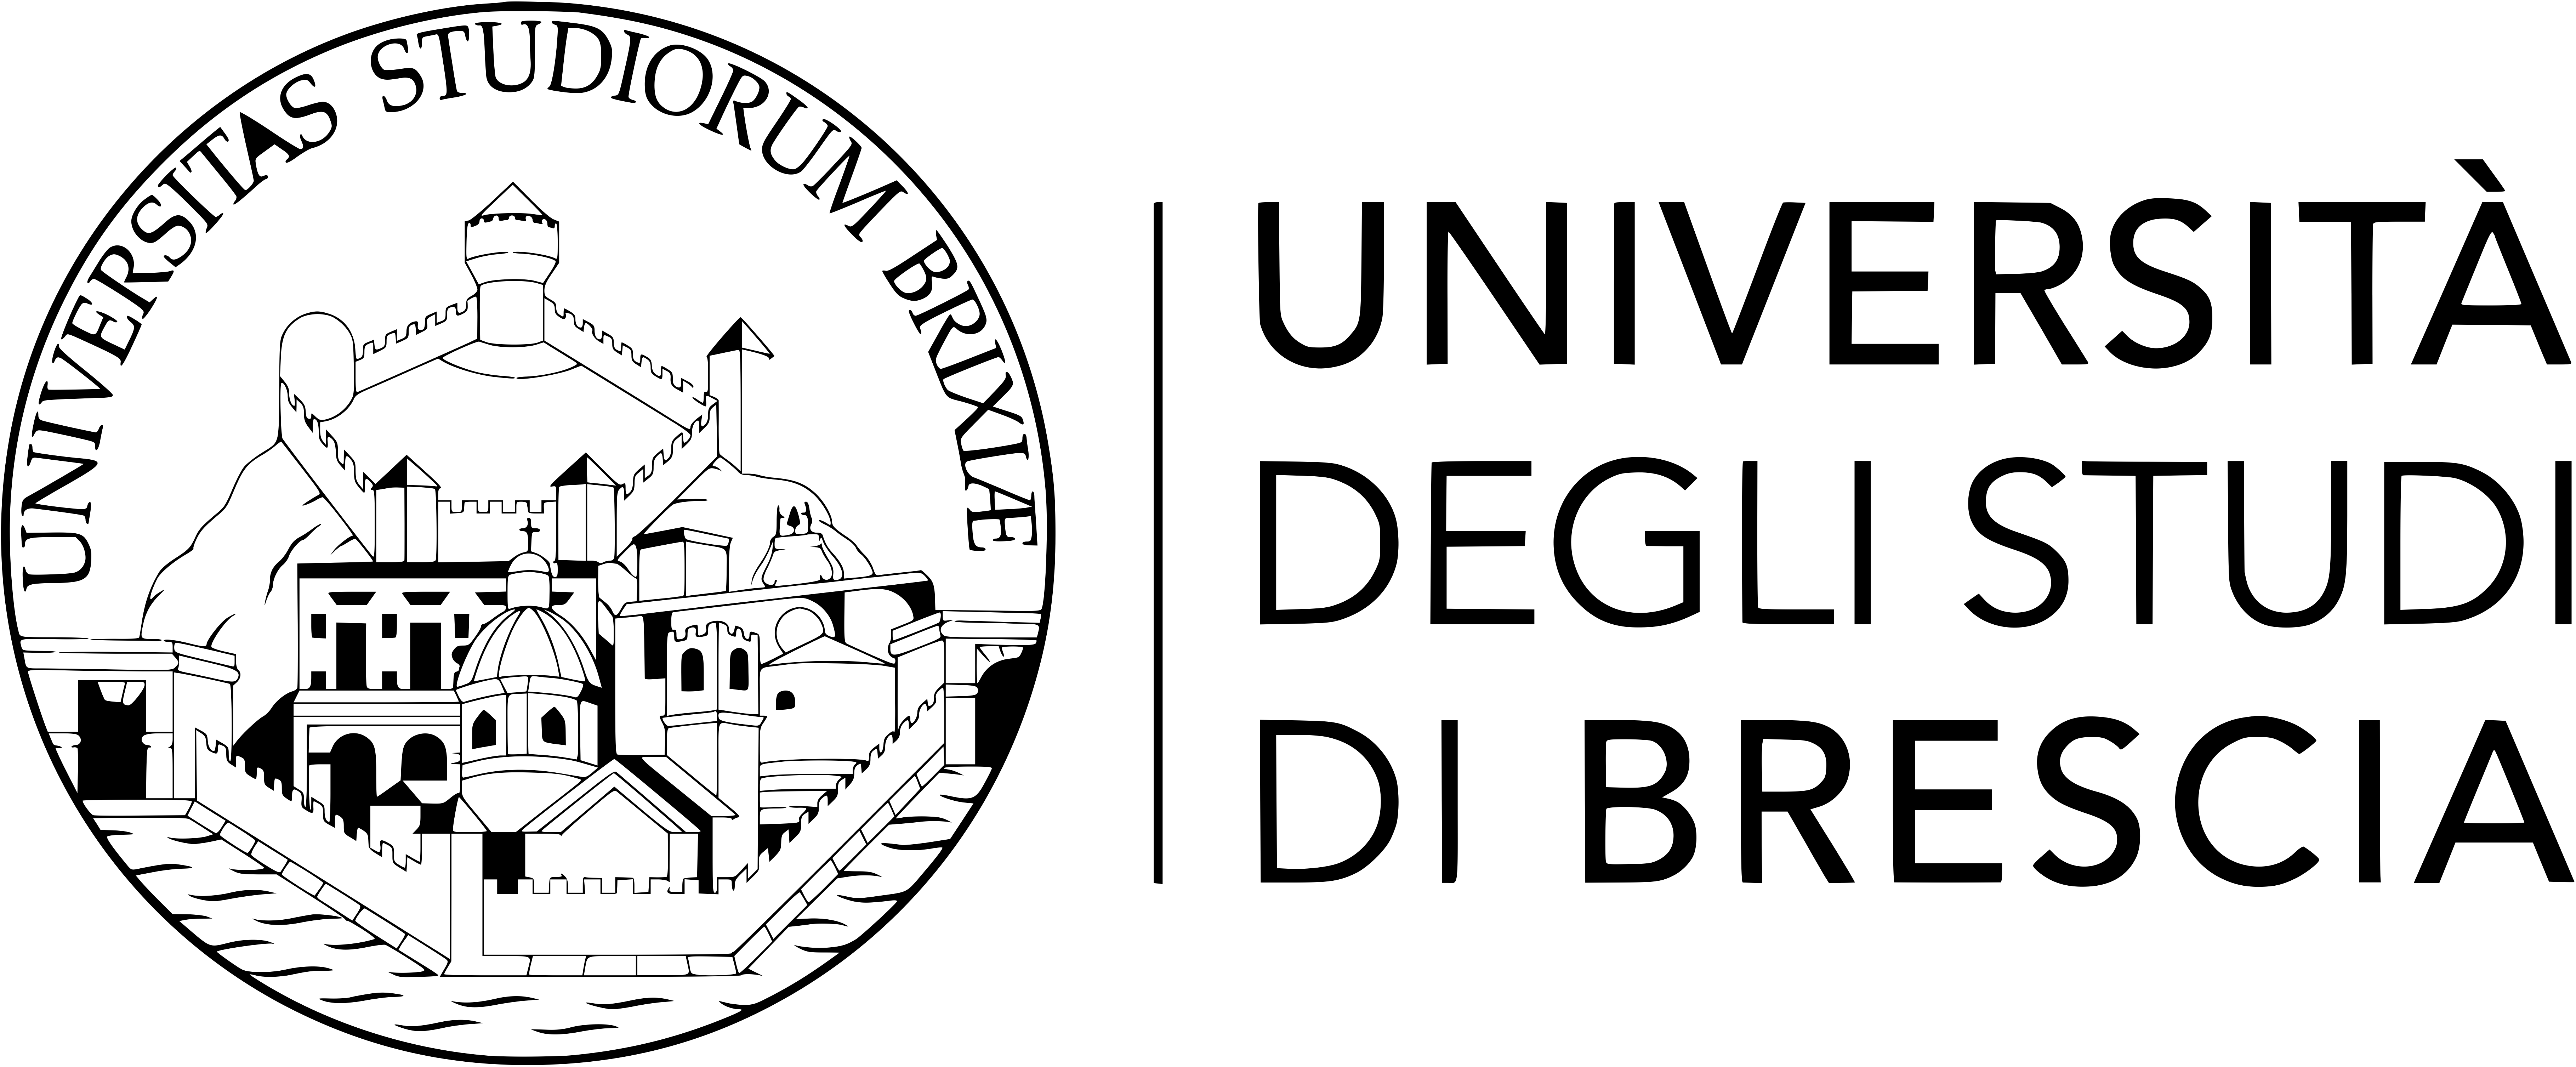
\includegraphics[width=0.5\textwidth]{src/images/unibs}\\%
}
\institute{Università degli Studi di Brescia}
\date{January 16, 2020}

%%%%%%%%%%%%%%%%%%%%%%%%%%%%%%%%%%%%%%%%%%%%%
% THEOREMS
%%%%%%%%%%%%%%%%%%%%%%%%%%%%%%%%%%%%%%%%%%%%%

%declare theorem, definitions, corollary, lemmas

%%%%%%%%%%%%%%%%%%%%%%%%%%%%%%%%%%%%%%%%%%%%%
% MAIN DOCUMENT
%%%%%%%%%%%%%%%%%%%%%%%%%%%%%%%%%%%%%%%%%%%%%

\begin{document}

%https://stackoverflow.com/a/3210406/1887602
\beamertemplatenavigationsymbolsempty

% add inputs
% \input{src/texs/...}
\begin{frame}[plain]
    \titlepage
\end{frame}
\section*{Introduction}

\begin{frame}{Introduction}
    Most Artificial Intelligence fields involve some sort of \textit{reasoning}: given some sort of \textit{knowledge} an agent reasons and acts rationally towards a \textit{goal}.

    Reasoning for a intelligent artificial agent can be \textit{static} or \textit{dynamic}:
    \begin{itemize}
        \item Static: solve a problem by exploiting some fixed knowledge;
        \item dynamic: solve a problem with mutable knowledge (\eg{} mantaining a property).
    \end{itemize}


    Many applications implicitly involve dynamic reasoning: 
    while such reasoning can be hard, it often is much faster \wrt{} static reasoning.
\end{frame}

\begin{frame}{Introduction (2): static reasoning example}

    \begin{block}{\vphantom{}}
        Given a directed graph $\graph{o} = \paircs{\graphv{}_{0}}{\graphe{o}_{0}}$, check if $\graph{o}$ has at least a cycle
    \end{block}

    \begin{figure}
        \begin{subfigure}{0.45\textwidth}
            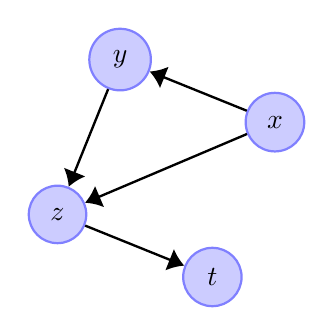
\begin{tikzpicture}
                \tikzstyle{vertex} = [shape=circle, fill=blue!20, draw=blue!50, thick, minimum size=2mm, inner sep=5pt, distance=1.7cm];

                \node[vertex](X) at (23:1.5cm) {$x$};
                \node[vertex](Y) at (113:1.5cm) {$y$};
                \node[vertex](Z) at (203:1.5cm) {$z$};
                \node[vertex](T) at (293:1.5cm) {$t$};

                \draw[-{Latex[length=2mm,width=3mm]}, line width=0.3mm]
                    (X) edge node[below]{} (Y)
                    (Y) edge node[left]{} (Z)
                    (X) edge node[below]{} (Z)

                    (Z) edge node[below]{} (T)
                ;
            \end{tikzpicture}
            \caption{$\graph{o}$ does not have a cycle}
        \end{subfigure}\hfill%
        \begin{subfigure}{0.45\textwidth}
            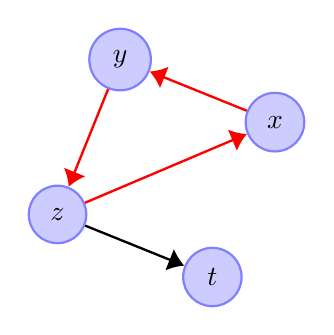
\begin{tikzpicture}
                \tikzstyle{vertex} = [shape=circle, fill=blue!20, draw=blue!50, thick, minimum size=2mm, inner sep=5pt, distance=1.7cm];

                \node[vertex](X) at (23:1.5cm) {$x$};
                \node[vertex](Y) at (113:1.5cm) {$y$};
                \node[vertex](Z) at (203:1.5cm) {$z$};
                \node[vertex](T) at (293:1.5cm) {$t$};

                \draw[-{Latex[length=2mm,width=3mm]}, line width=0.3mm]
                    (X) edge[color=red] node[below]{} (Y)
                    (Y) edge[color=red] node[left]{} (Z)
                    (Z) edge[color=red] node[below]{} (X)

                    (Z) edge node[below]{} (T)
                ;
            \end{tikzpicture}
            \caption{$\graph{o}$ has a cycle}
        \end{subfigure}
    \end{figure}

\end{frame}

\begin{frame}{Introduction (3): dynamic reasoning example}

    \begin{block}{\vphantom{}}
        Given a directed acyclic graph $\graph{o}_{0} = \paircs{\graphv{}_{0}}{\graphe{o}_{0}}$, check if $\graph{o}_{i+1} = \paircs{\graphv{}_{0}}{\graphe{o}_{i} \cup \{(u_i,v_i)\}} \; (u_i,v_i \in \graphv{}_{0}, (u_i,v_i) \not \in \graphe{o}_{i}, i = 0, 1, ..., k)$ has at least a cycle
    \end{block}

    \begin{figure}
        \centering
        \begin{subfigure}{0.29\textwidth}
            \centering
            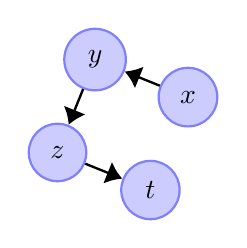
\begin{tikzpicture}
                \tikzstyle{vertex} = [shape=circle, fill=blue!20, draw=blue!50, thick, minimum size=2mm, inner sep=5pt, distance=1.7cm];

                \node[vertex](X) at (23:0.9cm) {$x$};
                \node[vertex](Y) at (113:0.9cm) {$y$};
                \node[vertex](Z) at (203:0.9cm) {$z$};
                \node[vertex](T) at (293:0.9cm) {$t$};

                \draw[-{Latex[length=2mm,width=3mm]}, line width=0.3mm]
                    (X) edge node[below]{} (Y)
                    (Y) edge node[left]{} (Z)
                    (Z) edge node[below]{} (T)
                ;
            \end{tikzpicture}
            \caption{$\graph{o}_{0}$ does not have a cycle}
        \end{subfigure}%
        \begin{subfigure}{0.04\textwidth}
            \centering
            \scalebox{1.5}{$\Rightarrow$}%
        \end{subfigure}%
        \begin{subfigure}{0.29\textwidth}
            \centering
            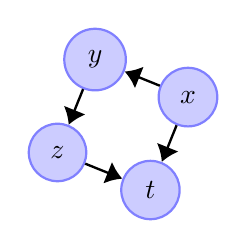
\begin{tikzpicture}
                \tikzstyle{vertex} = [shape=circle, fill=blue!20, draw=blue!50, thick, minimum size=2mm, inner sep=5pt, distance=1.7cm];

                \node[vertex](X) at (23:0.9cm) {$x$};
                \node[vertex](Y) at (113:0.9cm) {$y$};
                \node[vertex](Z) at (203:0.9cm) {$z$};
                \node[vertex](T) at (293:0.9cm) {$t$};

                \draw[-{Latex[length=2mm,width=3mm]}, line width=0.3mm]
                    (X) edge node[below]{} (Y)
                    (Y) edge node[left]{} (Z)
                    (Z) edge node[below]{} (T)
                    (X) edge node[below]{} (T)
                ;
            \end{tikzpicture}
            \caption{$\graph{o}_{1}$ does not have a cycle ($u_0 = x, v_0=t$)}
        \end{subfigure}%
        \begin{subfigure}{0.04\textwidth}
            \centering
            \scalebox{1.5}{$\Rightarrow$}%
        \end{subfigure}%
        \begin{subfigure}{0.29\textwidth}
            \centering
            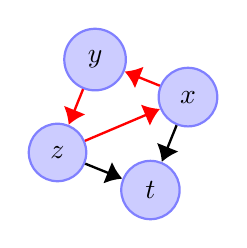
\begin{tikzpicture}
                \tikzstyle{vertex} = [shape=circle, fill=blue!20, draw=blue!50, thick, minimum size=2mm, inner sep=5pt, distance=1.7cm];

                \node[vertex](X) at (23:0.9cm) {$x$};
                \node[vertex](Y) at (113:0.9cm) {$y$};
                \node[vertex](Z) at (203:0.9cm) {$z$};
                \node[vertex](T) at (293:0.9cm) {$t$};

                \draw[-{Latex[length=2mm,width=3mm]}, line width=0.3mm]
                    (X) edge[color=red] node[below]{} (Y)
                    (Y) edge[color=red] node[left]{} (Z)
                    (Z) edge[color=red] node[below]{} (X)

                    (Z) edge node[below]{} (T)
                    (X) edge node[below]{} (T)
                ;
            \end{tikzpicture}
            \caption{$\graph{o}_{2}$ has a cycle ($u_1 = z, v_1=x$).}
        \end{subfigure}
    \end{figure}

    the dynamic problem can be solved with $k$ runs of the algorithm solving the static problem
    
    \begin{center}
    \textbf{however}
    \end{center}
    
    some knowledge is \textbf{not} exploited (\ie{} graphs are cumulative).
\end{frame}

\begin{frame}{Dynamic Graph-based Reasoning Systems}

    The thesis investigates two specific topics involving knowledge represented through graphs:

    \begin{itemize}
        \item \textbf{Consistency checking problem in temporal reasoning}: check if a network of constraint encoding temporal information is satisfiable;
        \item \textbf{\pathfinding{}}: given a graph, find the shortest-path from a start vertex to a target.
    \end{itemize}

    For both of them, we have considered a dynamic variant of the problem and we propose efficient algorithms for solving such variant. 
    The algorithms have been experimentally evaluated showing significant gains \wrt{} \stateofart{}.
\end{frame}

\begin{frame}{Talk Outline}

    The talk will be outlined as follows
    \begin{itemize}
        \item Decremental Consistency Checking Problem:
        \begin{itemize}
            \item Background (\CSPName{}, consistency, \tlGraphName{}, temporal algebras);
            \item motivation and problem definition;
            \item \DPASATAlgorithmName{} and \DOHSATAlgorithmName{};
            \item experimental results.
        \end{itemize}
        \item \SAPFEC{} Problem:
        \begin{itemize}
            \item Background (\pathfinding{}, \CPD{});
            \item motivation and problem definition;
            \item \CPDSearch{};
            \item experimental results.
        \end{itemize}
        \item Conclusion and future works.
    \end{itemize}
\end{frame}
\section*{Decremental Consistency Checking Problem}

\begin{frame}{Constraint Satisfactory Problem (\CSPName)}
    \begin{block}{Constraint Satisfactory Problem (\CSPName{})}%
		A CSP $\CSP{}$ consists of a finite set of \textit{variables} $\mathcal{V} = \{ x_1, x_2, ... x_n \}$; 
        each variable $x \in \mathcal{V}$ has associated a finite domain of values $Dom(x) = \{ v_1, ..., v_k\}$ and a finite set of constraints $\mathcal{C} = \{ C_1, ..., C_m \}$.
	\end{block}

    Example: Graph coloring

    \begin{minipage}{0.28\textwidth}
        \begin{figure}
            \centering
            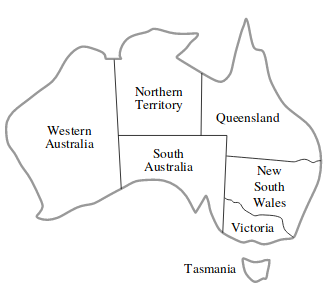
\includegraphics[width=1.0\textwidth]{{{src/images/temporal-reasoning/australia-map}}}
        \end{figure}
    \end{minipage}\hfill%
    \begin{minipage}{0.68\textwidth}
        \begin{equation*}
            \begin{split}
                \mathcal{V} & = \{ WA, NT, SA, Q, NSW, V, T \} \\
                Dom(x) & = \{ red, green, blue \}, \forall x \in \mathcal{V} \\
                \mathcal{C} & = \{ SA \not = WA, SA \not = NT, SA \not = Q, \\
                & \;\;\;\; SA \not = NSW, SA \not = V, \\
                & \;\;\;\; WA \not = NT, NT \not = Q, Q \not = NSW, \\
                & \;\;\;\; NSW \not = V \}
            \end{split}
        \end{equation*}
    \end{minipage}

\end{frame}

\begin{frame}{Constraint Graph}
    \CSPNames{} can be represented via \textit{constraint graphs}. 
    A \textit{solution} is a complete assignment of the variables which satisfies \textbf{all} constraints.

    \vspace{-8pt}
    \begin{minipage}{0.23\textwidth}
        \centering
        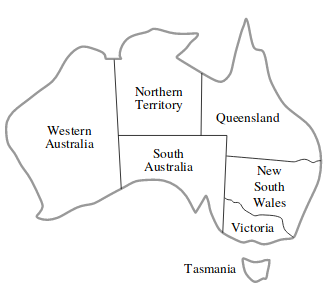
\includegraphics[width=1.0\textwidth]{{{src/images/temporal-reasoning/australia-map}}}
    \end{minipage}\hfill%
    \begin{minipage}{0.75\textwidth}
        \begin{equation*}
            \begin{split}
                \mathcal{V} & = \{ WA, NT, SA, Q, NSW, V, T \} \\
                Dom(x) & = \{ red, green, blue \}, \forall x \in \mathcal{V} \\
                \mathcal{C} & = \{ SA \not = WA, SA \not = NT, SA \not = Q, \\
                & \;\;\;\; SA \not = NSW, SA \not = V, WA \not = NT, \\
                & \;\;\;\; NT \not = Q, Q \not = NSW, NSW \not = V \}
            \end{split}
        \end{equation*}
    \end{minipage}\\
    \begin{minipage}{0.5\textwidth}
        \begin{figure}
            \centering
            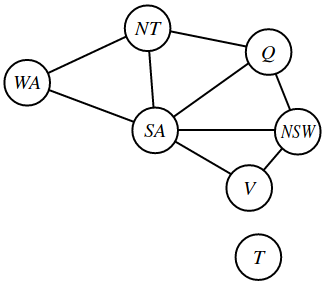
\includegraphics[width=0.5\textwidth]{src/images/temporal-reasoning/australia-graph}
            \caption{Constraint graph of \CSP{}.}
        \end{figure}
    \end{minipage}\hfill%
    \begin{minipage}{0.5\textwidth}
        \begin{figure}
            \centering
            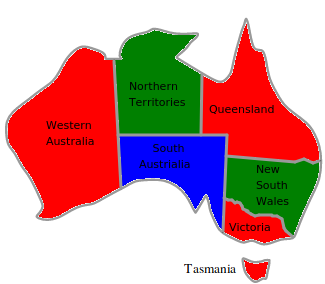
\includegraphics[width=0.5\textwidth]{src/images/temporal-reasoning/australia-map-colored}
            \caption{Representation of a solution of \CSP{}.}
        \end{figure}
    \end{minipage}
\end{frame}

\begin{frame}{Consistency}
    \begin{block}{Consistency}
		A CSP $\CSP{}$ is \textbf{satisfiable} (\textbf{consistent}) iff there is at least one solution 
        (\ie{} assignment of values to all the variables $\{x_i = v_i\}$ s.t. no constraint is violated).
	\end{block}

    \begin{figure}
        \centering
        \begin{subfigure}{0.48\textwidth}
            \centering
            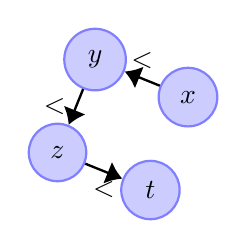
\begin{tikzpicture}
                \tikzstyle{vertex} = [shape=circle, fill=blue!20, draw=blue!50, thick, minimum size=2mm, inner sep=5pt, distance=1.7cm];

                \node[vertex](X) at (23:0.9cm) {$x$};
                \node[vertex](Y) at (113:0.9cm) {$y$};
                \node[vertex](Z) at (203:0.9cm) {$z$};
                \node[vertex](T) at (293:0.9cm) {$t$};

                \draw[-{Latex[length=2mm,width=3mm]}, line width=0.3mm]
                    (X) edge node[above]{$<$} (Y)
                    (Y) edge node[left]{$<$} (Z)
                    (Z) edge node[below]{$<$} (T)
                ;
            \end{tikzpicture}
            \caption{Constraint graph of a consistent \CSPName{}}
        \end{subfigure}\hfill%
        \begin{subfigure}{0.48\textwidth}
            \centering
            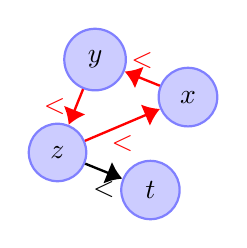
\begin{tikzpicture}
                \tikzstyle{vertex} = [shape=circle, fill=blue!20, draw=blue!50, thick, minimum size=2mm, inner sep=5pt, distance=1.7cm];

                \node[vertex](X) at (23:0.9cm) {$x$};
                \node[vertex](Y) at (113:0.9cm) {$y$};
                \node[vertex](Z) at (203:0.9cm) {$z$};
                \node[vertex](T) at (293:0.9cm) {$t$};

                \draw[-{Latex[length=2mm,width=3mm]}, line width=0.3mm]
                    (X) edge[color=red] node[above]{$<$} (Y)
                    (Y) edge[color=red] node[left]{$<$} (Z)
                    (Z) edge[color=red] node[below]{$<$} (X)
                    (Z) edge node[below]{$<$} (T)
                ;
            \end{tikzpicture}
            \caption{Constraint graph of an inconsistent \CSPName{}}
        \end{subfigure}
    \end{figure}

\end{frame}

\begin{frame}{Temporal \CSPNames{}}
    \begin{itemize}
        \item Focus on \TCSPNames{} (\ie{} \CSPNames{} where the variables represent timed events and each constraint involves a relation between 2 events);
        \item constraints: relations in Point Algebra (\PAName{}), Interval Algebra (\IAName{}) or its maximal tractable subalgebra,  \OrdHornName{}.
        \item variables: time points (for \PAName{}) or time intervals (for \IAName{});
        \item \IAName{}: $\bot$, 13 base relations and all their possible unions (\eg{} two intervals cannot overlap);
        \item \PAName{}: $<, =, >, \leq, \geq, \noteq{}, \top, \bot$ (\eg{} $x \noteq{} y$ means that the two events cannot occur at the same time); example of a \TCSPName{} over \PAName{}:
	\end{itemize}

    \begin{figure}
        \centering
        \begin{subfigure}{0.44\textwidth}
            \centering
            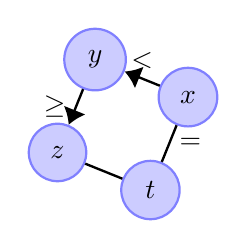
\begin{tikzpicture}
                \tikzstyle{vertex} = [shape=circle, fill=blue!20, draw=blue!50, thick, minimum size=2mm, inner sep=5pt, distance=1.7cm];

                \node[vertex](X) at (23:0.9cm) {$x$};
                \node[vertex](Y) at (113:0.9cm) {$y$};
                \node[vertex](Z) at (203:0.9cm) {$z$};
                \node[vertex](T) at (293:0.9cm) {$t$};

                \draw[-{Latex[length=2mm,width=3mm]}, line width=0.3mm]
                    (X) edge node[above]{$<$} (Y)
                    (Y) edge node[left]{$\geq$} (Z)
                ;

                \draw[-., line width=0.3mm]
                    (Z) edge node[below]{$\noteq{}$} (T)
                    (X) edge node[right]{$=$} (T)
                ;
            \end{tikzpicture}
        \end{subfigure}\hfill%
        \begin{subfigure}{0.1\textwidth}
            \centering
            $\xrightarrow{\mbox{\tlGraphName{}}}$
        \end{subfigure}\hfill%
        \begin{subfigure}{0.44\textwidth}
            \centering
            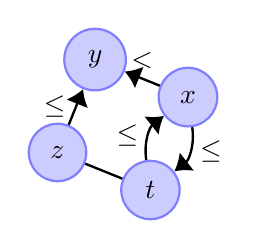
\begin{tikzpicture}
                \tikzstyle{vertex} = [shape=circle, fill=blue!20, draw=blue!50, thick, minimum size=2mm, inner sep=5pt, distance=1.7cm];

                \node[vertex](X) at (23:0.9cm) {$x$};
                \node[vertex](Y) at (113:0.9cm) {$y$};
                \node[vertex](Z) at (203:0.9cm) {$z$};
                \node[vertex](T) at (293:0.9cm) {$t$};

                \draw[-{Latex[length=2mm,width=3mm]}, line width=0.3mm]
                    (X) edge node[above]{$<$} (Y)
                    (Z) edge node[left]{$\leq$} (Y)
                    (X) edge[bend left] node[right]{$\leq$} (T)
                    (T) edge[bend left] node[left]{$\leq$} (X)
                ;

                \draw[-., line width=0.3mm]
                    (Z) edge node[below]{$\noteq{}$} (T)
                ;
            \end{tikzpicture}
        \end{subfigure}
    \end{figure}
\end{frame}

\begin{frame}{The Decremental Consistency Checking Problem: Motivation}
    \begin{figure}
        \centering
        \begin{subfigure}{1.0\textwidth}%
            \centering
            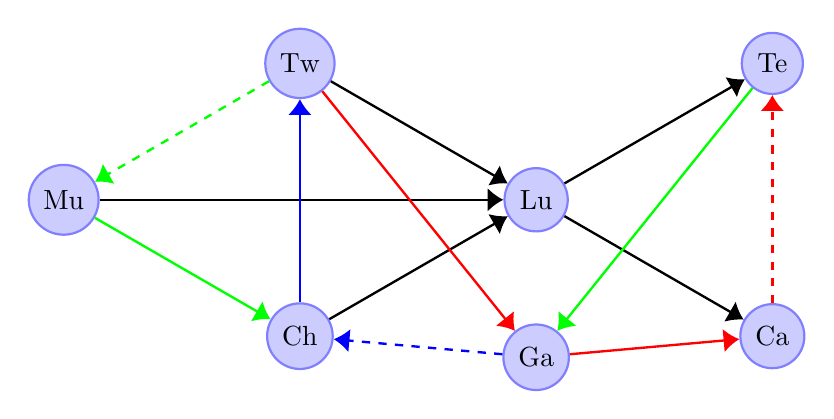
\begin{tikzpicture}
                \tikzstyle{vertex} = [
	shape=circle,  
	draw=blue!50, %draw the border to the node
	fill=blue!20, %fill the space of the node
	thick,
	minimum size=4mm, %minimum size of the nodes
	distance=1cm
];
\pgfarrowsdeclare{directEdge}{directEdge}{%
	\arrowsize=0.2pt
	\advance\arrowsize by .5\pgflinewidth
	\pgfarrowsleftextend{-4\arrowsize-.5\pgflinewidth}
	\pgfarrowsrightextend{.5\pgflinewidth}
}{%
	\arrowsize=1pt
	\advance\arrowsize by .5\pgflinewidth
	\pgfsetdash{}{0pt} % do not dash
	\pgfsetroundjoin % fix join
	\pgfsetroundcap % fix cap
	\pgfpathmoveto{\pgfpointorigin}
	\pgfpathlineto{\pgfpoint{-6\arrowsize}{2.2\arrowsize}}
	\pgfpathlineto{\pgfpoint{-6\arrowsize}{-2.2\arrowsize}}
	\pgfpathclose
	\pgfusepathqfill
}

\begin{scope}[scale=1.0,shift={(-3,0)}]
	\node[vertex](Tw) at (60:2.0cm) {Tw};
	\node[vertex](Mu) at (180:2.0cm) {Mu};
	\node[vertex](Ch) at (-60:2.0cm) {Ch};
\end{scope}

\begin{scope}[scale=1.0,shift={(3,0)}]
	\node[vertex](Lu) at (180:2.0cm) {Lu};
	\node[vertex](Ca) at (-60:2.0cm) {Ca};
	\node[vertex](Te) at (+60:2.0cm) {Te};
\end{scope}

\begin{scope}[scale=1.0,shift={(3,-2)}]
	\node[vertex](Ga) at (180:2.0cm) {Ga};
\end{scope}

%mandatory constraints
\draw[-{Latex[length=2mm,width=3mm]}, line width=0.3mm, color=black]
	(Tw) edge[] (Lu)
	(Ch) edge[] (Lu)
	(Mu) edge[] (Lu)
	(Lu) edge[] (Te)
	(Lu) edge[] (Ca)
;

%first tourist
\draw[-{Latex[length=2mm,width=3mm]}, line width=0.3mm, color=red]
	(Tw) edge[] (Ga)
	(Ga) edge[] (Ca)
	(Ca) edge[dashed] (Te)
;
	
%second tourist
\draw[-{Latex[length=2mm,width=3mm]}, line width=0.3mm, color=green]
	(Tw) edge[dashed] (Mu)
	(Mu) edge[] (Ch)
	(Te) edge[] (Ga)
;

%third tourist
\draw[-{Latex[length=2mm,width=3mm]}, line width=0.3mm, color=blue]
	(Ga) edge[dashed] (Ch)
	(Ch) edge[] (Tw)
;

            \end{tikzpicture}
        \end{subfigure}\\%
        \begin{subfigure}{1.00\textwidth}%
            \centering
            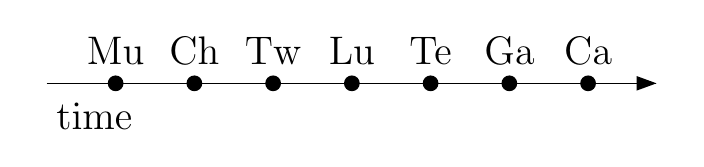
\begin{tikzpicture}
                \tikzstyle{vertex} = [
	shape=circle,  
	fill=black, %fill the space of the node
	thick,
	minimum size=2mm, %minimum size of the nodes
	inner sep=0pt,
	distance=2cm
];
\pgfarrowsdeclare{directEdge}{directEdge}{%
	\arrowsize=0.2pt
	\advance\arrowsize by .5\pgflinewidth
	\pgfarrowsleftextend{-4\arrowsize-.5\pgflinewidth}
	\pgfarrowsrightextend{.5\pgflinewidth}
}{%
	\arrowsize=1pt
	\advance\arrowsize by .5\pgflinewidth
	\pgfsetdash{}{0pt} % do not dash
	\pgfsetroundjoin % fix join
	\pgfsetroundcap % fix cap
	\pgfpathmoveto{\pgfpointorigin}
	\pgfpathlineto{\pgfpoint{-6\arrowsize}{2.2\arrowsize}}
	\pgfpathlineto{\pgfpoint{-6\arrowsize}{-2.2\arrowsize}}
	\pgfpathclose
	\pgfusepathqfill
}

\begin{scope}[scale=1.0,shift={(0,0)}]
	\node[draw=none,label distance=2.5cm,label=below right:\Large{time}](ZERO) at (0, 0) {};
	\node[vertex,label distance=1.6cm,label=above:\Large{Mu}](Mu) at (1, 0) {};
	\node[vertex,label distance=1.6cm,label=above:\Large{Ch}](Ch) at (2, 0) {};
	\node[vertex,label distance=1.6cm,label=above:\Large{Tw}](Tw) at (3, 0) {};
	\node[vertex,label distance=1.6cm,label=above:\Large{Lu}](Lu) at (4, 0) {};
	\node[vertex,label distance=1.6cm,label=above:\Large{Te}](Te) at (5, 0) {};
	\node[vertex,label distance=1.6cm,label=above:\Large{Ga}](Ga) at (6, 0) {};
	\node[vertex,label distance=1.6cm,label=above:\Large{Ca}](Ca) at (7, 0) {};
	\node[draw=none](INF) at (8, 0) {};
\end{scope}

\draw [-directEdge] (ZERO) to[] (INF);




            \end{tikzpicture}
        \end{subfigure}%
    \end{figure}
\end{frame}

\begin{frame}{Definition}
    Given:
	\begin{itemize}
		\item[-] \small{an \textbf{inconsistent temporal CSP} \CSP{} over a class of constraints $\mathcal{C}$};
		\item[-] \small{a \textbf{sequence} $\CSP{}_{0}, ..., \CSP{}_k$ of \TCSPNames{} over $\mathcal{C}$ such that $\CSP{}= \CSP{}_{0}$ and $\CSP{}_i$ is obtained from $\CSP{}_{i-1}$ by making one constraint relaxation in $\CSP{}_{i-1}$, for $i = 1, ..., k$};
	\end{itemize}
	\textbf{\color{blue} Decremental Consistency Checking} is the problem of \textit{iteratively deciding the consistency} of every $\CSP{}_i$ starting from $\CSP{}_1$ until $i = k$ or $\CSP{}_i$ becomes consistent.

    \makebox[\linewidth][c]{\begin{minipage}{1.3\textwidth}
        \begin{figure}
            \centering
            \begin{subfigure}[b]{0.23\textwidth}
                \centering
                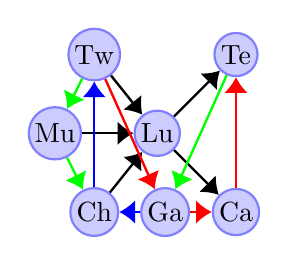
\begin{tikzpicture}
                    \tikzstyle{vertex} = [
	shape=circle,  
	draw=blue!50, %draw the border to the node
	fill=blue!20, %fill the space of the node
	thick,
	minimum size=1mm, %minimum size of the nodes
	distance=1cm,
	inner sep=1pt
];

\begin{scope}[scale=1.0,shift={(-1,0)}]
	\node[vertex](Tw) at (90:1.0cm) {Tw};
	\node[vertex](Mu) at (180:0.5cm) {Mu};
	\node[vertex](Ch) at (-90:1.0cm) {Ch};
\end{scope}

\begin{scope}[scale=1.0,shift={(0.8,0)}]
	\node[vertex](Lu) at (180:1.0cm) {Lu};
	\node[vertex](Ca) at (-90:1.0cm) {Ca};
	\node[vertex](Te) at (+90:1.0cm) {Te};
\end{scope}

\begin{scope}[scale=1.0,shift={(0.9,-1)}]
	\node[vertex](Ga) at (180:1.0cm) {Ga};
\end{scope}

%mandatory constraints
\draw[-{Latex[length=2mm,width=3mm]}, line width=0.3mm, color=black]
	(Tw) edge[] (Lu)
	(Ch) edge[] (Lu)
	(Mu) edge[] (Lu)
	(Lu) edge[] (Te)
	(Lu) edge[] (Ca)
;

%first tourist
\draw[-{Latex[length=2mm,width=3mm]}, line width=0.3mm, color=red]
	(Tw) edge[] (Ga)
	(Ga) edge[] (Ca)
	(Ca) edge[] (Te)
;
	
%second tourist
\draw[-{Latex[length=2mm,width=3mm]}, line width=0.3mm, color=green]
	(Tw) edge[] (Mu)
	(Mu) edge[] (Ch)
	(Te) edge[] (Ga)
;

%third tourist
\draw[-{Latex[length=2mm,width=3mm]}, line width=0.3mm, color=blue]
	(Ga) edge[] (Ch)
	(Ch) edge[] (Tw)
;

                \end{tikzpicture}
                \caption{$\CSP{}_{0}$}
            \end{subfigure}%
            \begin{subfigure}[b]{0.23\textwidth}
                \centering
                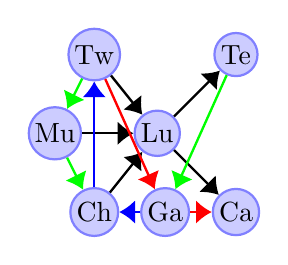
\begin{tikzpicture}
                    \tikzstyle{vertex} = [
	shape=circle,  
	draw=blue!50, %draw the border to the node
	fill=blue!20, %fill the space of the node
	thick,
	minimum size=1mm, %minimum size of the nodes
	distance=1cm,
	inner sep=1pt
];

\begin{scope}[scale=1.0,shift={(-1,0)}]
	\node[vertex](Tw) at (90:1.0cm) {Tw};
	\node[vertex](Mu) at (180:0.5cm) {Mu};
	\node[vertex](Ch) at (-90:1.0cm) {Ch};
\end{scope}

\begin{scope}[scale=1.0,shift={(0.8,0)}]
	\node[vertex](Lu) at (180:1.0cm) {Lu};
	\node[vertex](Ca) at (-90:1.0cm) {Ca};
	\node[vertex](Te) at (+90:1.0cm) {Te};
\end{scope}

\begin{scope}[scale=1.0,shift={(0.9,-1)}]
	\node[vertex](Ga) at (180:1.0cm) {Ga};
\end{scope}

%mandatory constraints
\draw[-{Latex[length=2mm,width=3mm]}, line width=0.3mm, color=black]
	(Tw) edge[] (Lu)
	(Ch) edge[] (Lu)
	(Mu) edge[] (Lu)
	(Lu) edge[] (Te)
	(Lu) edge[] (Ca)
;

%first tourist
\draw[-{Latex[length=2mm,width=3mm]}, line width=0.3mm, color=red]
	(Tw) edge[] (Ga)
	(Ga) edge[] (Ca)
;
	
%second tourist
\draw[-{Latex[length=2mm,width=3mm]}, line width=0.3mm, color=green]
	(Tw) edge[] (Mu)
	(Mu) edge[] (Ch)
	(Te) edge[] (Ga)
;

%third tourist
\draw[-{Latex[length=2mm,width=3mm]}, line width=0.3mm, color=blue]
	(Ga) edge[] (Ch)
	(Ch) edge[] (Tw)
;

                \end{tikzpicture}
                \caption{$\CSP{}_{1}$}
            \end{subfigure}%
            \begin{subfigure}[b]{0.23\textwidth}
                \centering
                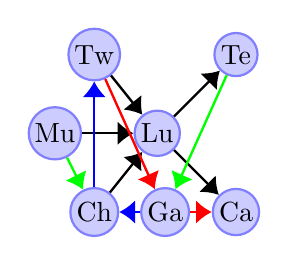
\begin{tikzpicture}
                    \tikzstyle{vertex} = [
	shape=circle,  
	draw=blue!50, %draw the border to the node
	fill=blue!20, %fill the space of the node
	thick,
	minimum size=1mm, %minimum size of the nodes
	distance=1cm,
	inner sep=1pt
];

\begin{scope}[scale=1.0,shift={(-1,0)}]
	\node[vertex](Tw) at (90:1.0cm) {Tw};
	\node[vertex](Mu) at (180:0.5cm) {Mu};
	\node[vertex](Ch) at (-90:1.0cm) {Ch};
\end{scope}

\begin{scope}[scale=1.0,shift={(0.8,0)}]
	\node[vertex](Lu) at (180:1.0cm) {Lu};
	\node[vertex](Ca) at (-90:1.0cm) {Ca};
	\node[vertex](Te) at (+90:1.0cm) {Te};
\end{scope}

\begin{scope}[scale=1.0,shift={(0.9,-1)}]
	\node[vertex](Ga) at (180:1.0cm) {Ga};
\end{scope}

%mandatory constraints
\draw[-{Latex[length=2mm,width=3mm]}, line width=0.3mm, color=black]
	(Tw) edge[] (Lu)
	(Ch) edge[] (Lu)
	(Mu) edge[] (Lu)
	(Lu) edge[] (Te)
	(Lu) edge[] (Ca)
;

%first tourist
\draw[-{Latex[length=2mm,width=3mm]}, line width=0.3mm, color=red]
	(Tw) edge[] (Ga)
	(Ga) edge[] (Ca)
;
	
%second tourist
\draw[-{Latex[length=2mm,width=3mm]}, line width=0.3mm, color=green]
	(Mu) edge[] (Ch)
	(Te) edge[] (Ga)
;

%third tourist
\draw[-{Latex[length=2mm,width=3mm]}, line width=0.3mm, color=blue]
	(Ga) edge[] (Ch)
	(Ch) edge[] (Tw)
;

                \end{tikzpicture}
                \caption{$\CSP{}_{2}$}
            \end{subfigure}%
            \begin{subfigure}[b]{0.23\textwidth}
                \centering
                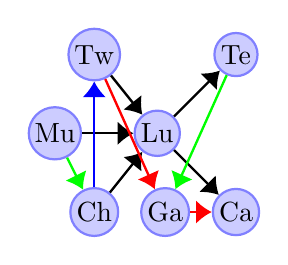
\begin{tikzpicture}
                    \tikzstyle{vertex} = [
	shape=circle,  
	draw=blue!50, %draw the border to the node
	fill=blue!20, %fill the space of the node
	thick,
	minimum size=1mm, %minimum size of the nodes
	distance=1cm,
	inner sep=1pt
];

\begin{scope}[scale=1.0,shift={(-1,0)}]
	\node[vertex](Tw) at (90:1.0cm) {Tw};
	\node[vertex](Mu) at (180:0.5cm) {Mu};
	\node[vertex](Ch) at (-90:1.0cm) {Ch};
\end{scope}

\begin{scope}[scale=1.0,shift={(0.8,0)}]
	\node[vertex](Lu) at (180:1.0cm) {Lu};
	\node[vertex](Ca) at (-90:1.0cm) {Ca};
	\node[vertex](Te) at (+90:1.0cm) {Te};
\end{scope}

\begin{scope}[scale=1.0,shift={(0.9,-1)}]
	\node[vertex](Ga) at (180:1.0cm) {Ga};
\end{scope}

%mandatory constraints
\draw[-{Latex[length=2mm,width=3mm]}, line width=0.3mm, color=black]
	(Tw) edge[] (Lu)
	(Ch) edge[] (Lu)
	(Mu) edge[] (Lu)
	(Lu) edge[] (Te)
	(Lu) edge[] (Ca)
;

%first tourist
\draw[-{Latex[length=2mm,width=3mm]}, line width=0.3mm, color=red]
	(Tw) edge[] (Ga)
	(Ga) edge[] (Ca)
;
	
%second tourist
\draw[-{Latex[length=2mm,width=3mm]}, line width=0.3mm, color=green]
	(Mu) edge[] (Ch)
	(Te) edge[] (Ga)
;

%third tourist
\draw[-{Latex[length=2mm,width=3mm]}, line width=0.3mm, color=blue]
	(Ch) edge[] (Tw)
;

                \end{tikzpicture}
                \caption{$\CSP{}_{3}$}
            \end{subfigure}
        \end{figure}
    \end{minipage}}
\end{frame}

\begin{frame}{\PSATProblemName{}}
    How to solve the problem of \textit{statically} checking the consistency of a \TCSPName{} \CSP{} over \PAName{} (\PSATProblemName{})?

    \begin{itemize}
        \item Compute the \textit{Strongly Connected Components} (\SCCNames{}) of the \tlGraphName{} of \CSP{};
        \item Edge labeled either with $<$ or $\noteq{}$ is in a \SCCName{} subgraph $\Leftrightarrow$ \CSP{} inconsistent;
    \end{itemize}

    \begin{figure}
        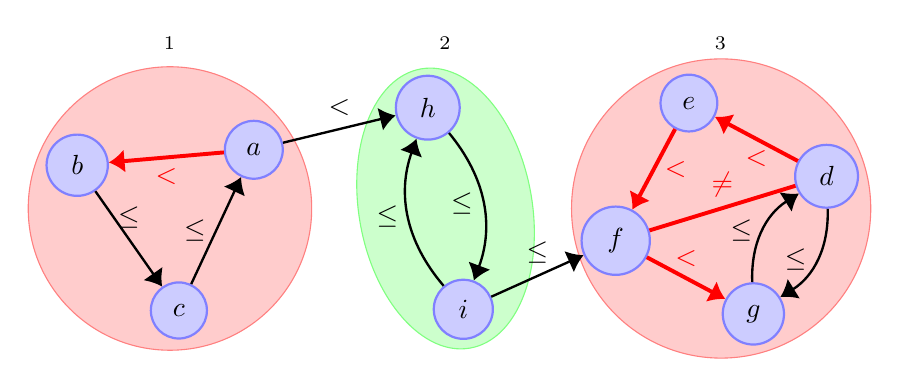
\begin{tikzpicture}
            \tikzstyle{vertex}=[shape=circle, fill=blue!20, draw=blue!50, thick, minimum size=2mm, inner sep=5pt, distance=1.7cm];

            \begin{scope}[scale=1.0, shift={(0,0)}]
                \node at (0,2.1cm) {$\SCC{}_{1}$};
                \draw[fill=red!20, draw=red!50] (0,0) circle (1.8cm);
                \node[vertex](A) at (35:1.3cm) {$a$};
                \node[vertex](B) at (155:1.3cm) {$b$};
                \node[vertex](C) at (275:1.3cm) {$c$};
            \end{scope}

            \begin{scope}[scale=1.0, shift={(7,0)}]
                \node at (0,2.1cm) {$\SCC{}_{3}$};
                \draw[fill=red!20, draw=red!50] (0,0) circle (1.9cm);
                \node[vertex](D) at (17:1.4cm) {$d$};
                \node[vertex](E) at (107:1.4cm) {$e$};
                \node[vertex](F) at (197:1.4cm) {$f$};
                \node[vertex](G) at (287:1.4cm) {$g$};
            \end{scope}

            \begin{scope}[scale=1.0, shift={(3.5,0)}]
                \node at (0,2.1cm) {$\SCC{}_{2}$};
                \draw[fill=green!20, draw=green!50, rotate=10] (0,0) circle (1.1cm and 1.8cm);
                \node[vertex](H) at (100:1.3cm) {$h$};
                \node[vertex](I) at (280:1.3cm) {$i$};
            \end{scope}

            \draw[-{Latex[length=2mm,width=3mm]}, line width=0.3mm]
                (A) edge[color=red, line width=0.5mm] node[below] {$<$} (B)
                (B) edge node[above] {$\leq$} (C)
                (C) edge node[left] {$\leq$} (A)
            ;

            \draw[-{Latex[length=2mm,width=3mm]}, line width=0.3mm]
                (D) edge[color=red, line width=0.5mm] node[below] {$<$} (E)
                (E) edge[color=red, line width=0.5mm] node[right] {$<$} (F)
                (F) edge[color=red, line width=0.5mm] node[above] {$<$} (G)
                (G) edge[bend left] node[left] {$\leq$} (D)
                (D) edge[bend left] node[left] {$\leq$} (G)
            ;

            \draw[-.]
                (F) edge[color=red, line width=0.5mm] node[above] {$\not =$} (D)
            ;

            \draw[-{Latex[length=2mm,width=3mm]}, line width=0.3mm]
                (H) edge[bend left] node[left] {$\leq$} (I)
                (I) edge[bend left] node[left] {$\leq$} (H)
            ;

            \draw[-{Latex[length=2mm,width=3mm]}, line width=0.3mm]
                (A) edge node[above, yshift=1pt] {$<$} (H)
                (I) edge node[above, yshift=1pt] {$\leq$} (F)
            ;
        \end{tikzpicture}
    \end{figure}
\end{frame}
\section*{\SAPFEC{}}

\begin{frame}{General idea of \Pathfinding{}}

    \begin{block}{\Pathfinding{}}
        Given a weighted directed graph $\graph{o} = \paircs{\graphv{}}{\graphe{o}}$, $s, t \in \graphv{}$, \pathfinding{} is the task of computing a shortest-path from $s$ to $t$.
    \end{block}

    \begin{figure}
        \centering
        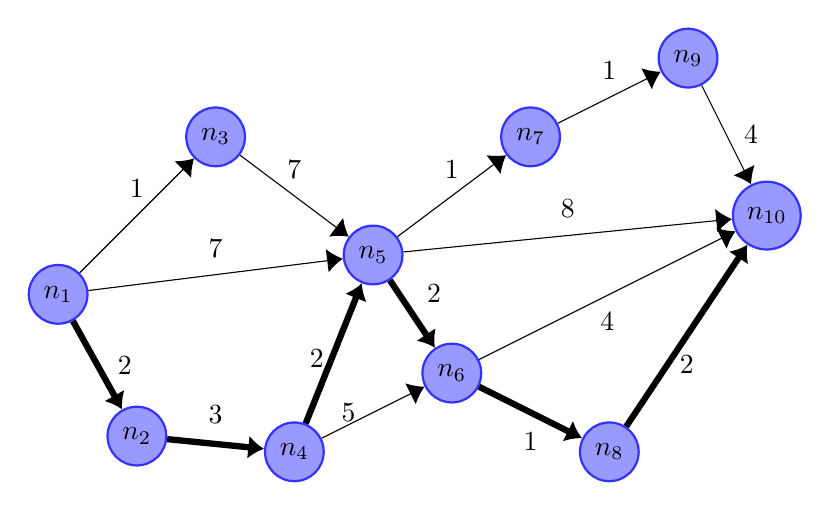
\begin{tikzpicture}
            \tikzset{Node/.style={circle, thick, draw=blue!80, fill=blue!40, minimum size=0.5cm}}
            \tikzset{OptimalPath/.style={circle, thick, draw=blue!80, fill=blue!40, minimum size=0.5cm}}

            \node[Node](N01) at (1,5) {$n_{1}$};
            \node[Node](N02) at (2,3.2) {$n_{2}$};
            \node[Node](N03) at (3,7) {$n_{3}$};
            \node[Node](N04) at (4,3) {$n_{4}$};
            \node[Node](N05) at (5,5.5) {$n_{5}$};
            \node[Node](N06) at (6,4) {$n_{6}$};
            \node[Node](N07) at (7,7) {$n_{7}$};
            \node[Node](N08) at (8,3) {$n_{8}$};
            \node[Node](N09) at (9,8) {$n_{9}$};
            \node[Node](N10) at (10,6) {$n_{10}$};

            \draw[-{Latex[length=2mm,width=3mm]}]
                (N01) edge node[above=1mm]{$7$} (N05) 
                (N01) edge node[above=1mm]{$1$} (N03) 
                (N03) edge node[above=1mm]{$7$} (N05)
                (N05) edge node[above=1mm]{$8$} (N10)
                (N04) edge node[left=1mm]{$5$} (N06)
                (N05) edge node[above=1mm]{$1$} (N07)
                (N07) edge node[above=1mm]{$1$} (N09)
                (N09) edge node[right=1mm]{$4$} (N10)
                (N06) edge node[below=1mm]{$4$} (N10)
            ;
            \draw[-{Latex[length=2mm,width=3mm]}, line width=0.8mm]
                (N01) edge node[right=1mm]{$2$} (N02) 
                (N02) edge node[above=1mm]{$3$} (N04)
                (N04) edge node[pos=0.2,above=2mm]{$2$} (N05)
                (N05) edge node[pos=0.2,right=2mm]{$2$} (N06)
                (N06) edge node[below=1mm]{$1$} (N08)
                (N08) edge node[below=1mm]{$2$} (N10)
                ;
        \end{tikzpicture}
    \end{figure}

\end{frame}

\begin{frame}{Compressed Path Database (\CPD{}) [Strasser 2014 et al.]}

    \vspace{-9pt}
    \begin{block}{}
        Given a graph, a \CPD{} is a data structure that efficiently stores the first edge of an optimal path from any node $s$ towards any node $t$.
    \end{block}

    \vspace{-2pt}
    \begin{minipage}{0.33\textwidth}
        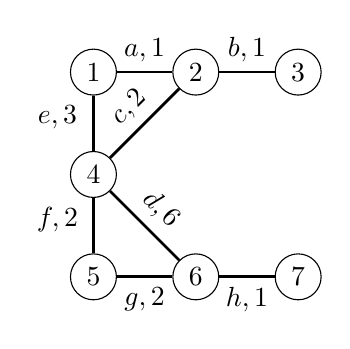
\begin{tikzpicture}
            \tikzset{Vertex/.style={%
                    shape=circle,%
                    draw=black,%
                    minimum size=10pt,%
                    radius=1cm,%
                    inner sep=3pt,%
                    node distance=1.3cm,%
                }}
        
                \node[Vertex] (1) {$1$};
                \node[Vertex, right of=1] (2) {$2$};
                \node[Vertex, right of=2] (3) {$3$};
                \node[Vertex, below of=1] (4) {$4$};
                \node[Vertex, below of=4] (5) {$5$};
                \node[Vertex, right of=5] (6) {$6$};
                \node[Vertex, right of=6] (7) {$7$};
        
                \path (1) edge[-,line width=1pt] node[above]{$a,1$} (2);
                \path (2) edge[-,line width=1pt] node[above]{$b,1$} (3);
                \path (4) edge[-,line width=1pt] node[above,sloped]{$c,2$} (2);
                \path (4) edge[-,line width=1pt] node[above,sloped]{$d,6$} (6);
                \path (4) edge[-,line width=1pt] node[above,xshift=-13pt,yshift=-6pt]{$e,3$} (1);
                \path (4) edge[-,line width=1pt] node[above,xshift=-13pt, yshift=-6pt]{$f,2$} (5);
                \path (5) edge[-,line width=1pt] node[below]{$g,2$} (6);
                \path (6) edge[-,line width=1pt] node[below]{$h,1$} (7);
        \end{tikzpicture}%
        \begin{center}%
            \vspace{-13pt}%
            $(s,t) = (2, 6)$%
        \end{center}
    \end{minipage}\hfill%
    \begin{minipage}{0.50\textwidth}
        \begin{center}
            \begin{minipage}{1.0\textwidth}
                \begin{minipage}{0.5\textwidth}
                    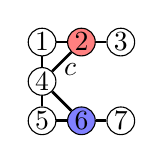
\begin{tikzpicture}
                        \tikzset{Vertex/.style={%
                                shape=circle,%
                                draw=black,%
                                minimum size=10pt,%
                                inner sep=0pt,%
                                node distance=0.5cm,%
                            }}
                    
                            \node[Vertex] (1) {$1$};
                            \node[Vertex, fill=red!50, right of=1] (2) {$2$};
                            \node[Vertex, right of=2] (3) {$3$};
                            \node[Vertex, below of=1] (4) {$4$};
                            \node[Vertex, below of=4] (5) {$5$};
                            \node[Vertex, fill=blue!50, right of=5] (6) {$6$};
                            \node[Vertex, right of=6] (7) {$7$};
                    
                            \path (1) edge[-,line width=1pt] (2);
                            \path (2) edge[-,line width=1pt] (3);
                            \path (4) edge[-,line width=1pt] node[xshift=3pt, yshift=3pt, below]{$c$} (2);
                            \path (4) edge[-,line width=1pt] (6);
                            \path (4) edge[-,line width=1pt] (1);
                            \path (4) edge[-,line width=1pt] (5);
                            \path (5) edge[-,line width=1pt] (6);
                            \path (6) edge[-,line width=1pt] (7);
                    \end{tikzpicture}
                \end{minipage}\hfill%
                \begin{minipage}{0.5\textwidth}
                    $CPD[2,6] = c$
                \end{minipage}

                \begin{minipage}{0.5\textwidth}
                    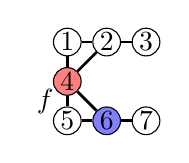
\begin{tikzpicture}
                        \tikzset{Vertex/.style={%
                                shape=circle,%
                                draw=black,%
                                minimum size=10pt,%
                                inner sep=0pt,%
                                node distance=0.5cm,%
                            }}
                    
                            \node[Vertex] (1) {$1$};
                            \node[Vertex, right of=1] (2) {$2$};
                            \node[Vertex, right of=2] (3) {$3$};
                            \node[Vertex, fill=red!50, below of=1] (4) {$4$};
                            \node[Vertex, below of=4] (5) {$5$};
                            \node[Vertex, fill=blue!50, right of=5] (6) {$6$};
                            \node[Vertex, right of=6] (7) {$7$};
                    
                            \path (1) edge[-,line width=1pt] (2);
                            \path (2) edge[-,line width=1pt] (3);
                            \path (4) edge[-,line width=1pt] (2);
                            \path (4) edge[-,line width=1pt] (6);
                            \path (4) edge[-,line width=1pt] (1);
                            \path (4) edge[-,line width=1pt] node[xshift=-8pt]{$f$} (5);
                            \path (5) edge[-,line width=1pt] (6);
                            \path (6) edge[-,line width=1pt] (7);
                    \end{tikzpicture}
                \end{minipage}\hfill%
                \begin{minipage}{0.5\textwidth}
                    $CPD[4,6] = f$
                \end{minipage}

                \begin{minipage}{0.5\textwidth}
                    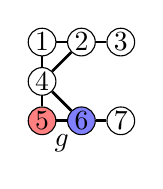
\begin{tikzpicture}
                        \tikzset{Vertex/.style={%
                                shape=circle,%
                                draw=black,%
                                minimum size=10pt,%
                                inner sep=0pt,%
                                node distance=0.5cm,%
                            }}
                    
                            \node[Vertex] (1) {$1$};
                            \node[Vertex, right of=1] (2) {$2$};
                            \node[Vertex, right of=2] (3) {$3$};
                            \node[Vertex, below of=1] (4) {$4$};
                            \node[Vertex, fill=red!50, below of=4] (5) {$5$};
                            \node[Vertex, fill=blue!50, right of=5] (6) {$6$};
                            \node[Vertex, right of=6] (7) {$7$};
                    
                            \path (1) edge[-,line width=1pt] (2);
                            \path (2) edge[-,line width=1pt] (3);
                            \path (4) edge[-,line width=1pt] (2);
                            \path (4) edge[-,line width=1pt] (6);
                            \path (4) edge[-,line width=1pt] (1);
                            \path (4) edge[-,line width=1pt] (5);
                            \path (5) edge[-,line width=1pt] node[yshift=-8pt]{$g$} (6);
                            \path (6) edge[-,line width=1pt] (7);
                    \end{tikzpicture}
                \end{minipage}\hfill%
                \begin{minipage}{0.5\textwidth}
                    $CPD[5,6] = g$
                \end{minipage}
            \end{minipage}

        \end{center}     
    \end{minipage}

    \vspace{-9pt}
    \begin{coloredBlock}{\CPDPathName{}}[OliveGreen][white]
        Given a graph $G$ and its \CPD{}, source node $s$ and target node $t$, 
        the $\CPDPath{s}{t}$ is the path obtained by concatenating edge $\CPD{}[s, t]$ with $\CPDPath{sink(\CPD{}[s, t])}{t}$ if $s \not = t$; the empty path otherwise.
    \end{coloredBlock}
\end{frame}

\begin{frame}{\A*{} [Nilsson et al., 1972]}
    \begin{block}{\A*{}}
        Given a (usually large) weighted directed graph representing a search space, an initial state $s$ and a set of goal states $T$, 
        the search algorithm \A*{} looks for the shortest path by iteratively expanding the best node 
    \end{block}
\end{frame}
% see https://tex.stackexchange.com/a/208409/145331
\begin{frame}[fragile]{\SAPFEC{} problem}

    \only<1>{
        \begin{center}
            \textbf{Original Map}

            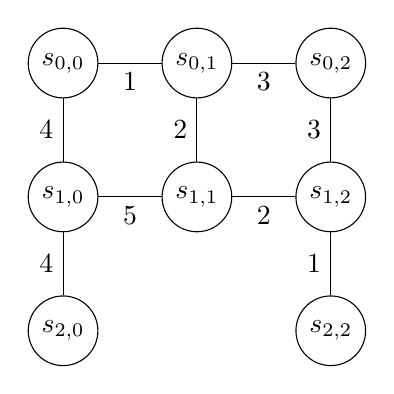
\begin{tikzpicture}
                \tikzset{Vertex/.style={%
                    shape=circle,%
                    draw=black,%
                    minimum size=10pt,%
                    radius=1cm,%
                    inner sep=3pt,%
                    node distance=1.7cm,%
                }}
        
                \node[Vertex] (v00) at (0,0) {$s_{0,0}$};
                \node[Vertex, right of=v00] (v01) {$s_{0,1}$};
                \node[Vertex, right of=v01] (v02) {$s_{0,2}$};
                \node[Vertex, below of=v00] (v10) {$s_{1,0}$};
                \node[Vertex, right of=v10] (v11) {$s_{1,1}$};
                \node[Vertex, right of=v11] (v12) {$s_{1,2}$};
                \node[Vertex, below of=v10] (v20) {$s_{2,0}$};
                \node[Vertex, below of=v12] (v22) {$s_{2,2}$};
        
                \path (v00) edge[-.] node[below]{1} (v01);
                \path (v01) edge[-.] node[below]{3} (v02);
                \path (v10) edge[-.] node[below]{5} (v11);
                \path (v11) edge[-.] node[below]{2} (v12);
                \path (v00) edge[-.] node[left]{4} (v10);
                \path (v10) edge[-.] node[left]{4} (v20);
                \path (v01) edge[-.] node[left]{2} (v11);
                \path (v02) edge[-.] node[left]{3} (v12);
                \path (v12) edge[-.] node[left]{1} (v22);
            \end{tikzpicture}
        \end{center}
    }%
    \only<2>{
        \begin{center}
            \textbf{Original Map}

            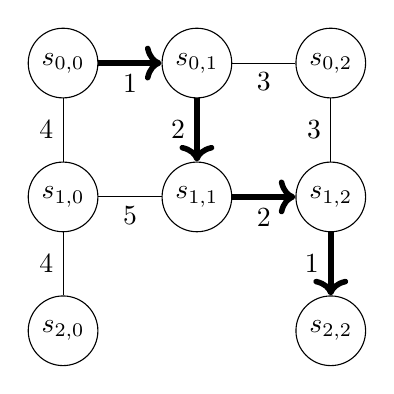
\begin{tikzpicture}
                \tikzset{Vertex/.style={%
                    shape=circle,%
                    draw=black,%
                    minimum size=10pt,%
                    radius=1cm,%
                    inner sep=3pt,%
                    node distance=1.7cm,%
                }}
        
                \node[Vertex] (v00) at (0,0) {$s_{0,0}$};
                \node[Vertex, right of=v00] (v01) {$s_{0,1}$};
                \node[Vertex, right of=v01] (v02) {$s_{0,2}$};
                \node[Vertex, below of=v00] (v10) {$s_{1,0}$};
                \node[Vertex, right of=v10] (v11) {$s_{1,1}$};
                \node[Vertex, right of=v11] (v12) {$s_{1,2}$};
                \node[Vertex, below of=v10] (v20) {$s_{2,0}$};
                \node[Vertex, below of=v12] (v22) {$s_{2,2}$};
        
                \path (v00) edge[->,line width=2pt] node[below]{1} (v01);
                \path (v01) edge[-.] node[below]{3} (v02);
                \path (v10) edge[-.] node[below]{5} (v11);
                \path (v11) edge[->,line width=2pt] node[below]{2} (v12);
                \path (v00) edge[-.] node[left]{4} (v10);
                \path (v10) edge[-.] node[left]{4} (v20);
                \path (v01) edge[->,line width=2pt] node[left]{2} (v11);
                \path (v02) edge[-.] node[left]{3} (v12);
                \path (v12) edge[->,line width=2pt] node[left]{1} (v22);
            \end{tikzpicture}

            $$s_{0,0} \rightarrow s_{0,1} \rightarrow s_{1,1} \rightarrow s_{1,2} \rightarrow s_{2,2}$$
        \end{center}
    }%
    \only<3>{
        \begin{center}
            \textbf{Perturbated Map}

            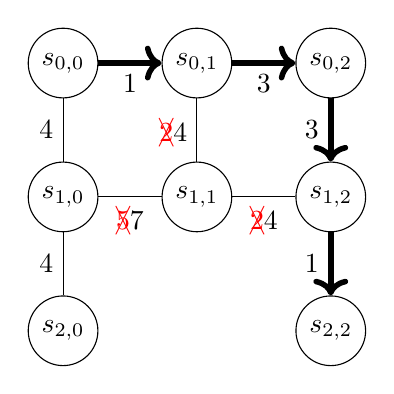
\begin{tikzpicture}
                \tikzset{Vertex/.style={%
                    shape=circle,%
                    draw=black,%
                    minimum size=10pt,%
                    radius=1cm,%
                    inner sep=3pt,%
                    node distance=1.7cm,%
                }}
        
                \node[Vertex] (v00) at (0,0) {$s_{0,0}$};
                \node[Vertex, right of=v00] (v01) {$s_{0,1}$};
                \node[Vertex, right of=v01] (v02) {$s_{0,2}$};
                \node[Vertex, below of=v00] (v10) {$s_{1,0}$};
                \node[Vertex, right of=v10] (v11) {$s_{1,1}$};
                \node[Vertex, right of=v11] (v12) {$s_{1,2}$};
                \node[Vertex, below of=v10] (v20) {$s_{2,0}$};
                \node[Vertex, below of=v12] (v22) {$s_{2,2}$};
        
                \path (v00) edge[->,line width=2pt] node[below]{1} (v01);
                \path (v01) edge[->,line width=2pt] node[below]{3} (v02);
                \path (v10) edge[-.] node[below]{{\color{red} \xcancel{5}}{7}} (v11);
                \path (v11) edge[-.] node[below]{{\color{red} \xcancel{2}}{4}} (v12);
                \path (v00) edge[-.] node[left]{4} (v10);
                \path (v10) edge[-.] node[left]{4} (v20);
                \path (v01) edge[-.] node[left]{{\color{red} \xcancel{2}}{4}} (v11);
                \path (v02) edge[->,line width=2pt] node[left]{3} (v12);
                \path (v12) edge[->,line width=2pt] node[left]{1} (v22);
            \end{tikzpicture}

            $$s_{0,0} \rightarrow s_{0,1} \rightarrow s_{0,2} \rightarrow s_{1,2} \rightarrow s_{2,2}$$
        \end{center}
    }
    
\end{frame}

\begin{frame}{\SAPFEC{} context}
    \begin{itemize}
        \item Path planning episodes are independent;
        \item each episode has fixed start and target locations;
        \item graph map is known a priori.
    \end{itemize}
    
    \medskip
    Map edge costs changes (\textit{perturbations}):
    \begin{itemize}
        \item[-] Distribution over map unknown a priori;
        \item[-] \textbf{only increase} original edge costs (\eg{} routing in road networks, videogames);
        \item[-] detected at the beginning of each path planning episode and then assumed fixed.
    \end{itemize}
\end{frame}


\begin{frame}{\CPDSearch{} [Bono, Gerevini, Harabor, Stuckey, 2019]}
    \vspace{-8pt}
    \begin{block}{\CPDSearch{}}
        \A{} variant yielding bounded suboptimal solutions where \CPDPathsName{} are exploited for searching the perturbated map (for brevity, here we focus on the optimal working mode)
    \end{block}

    $s$, $t$ : start and target of path finding instance;
    
    $n$: a search node expanded during \CPDSearch{};

    \begin{coloredBlock}{Property}[OliveGreen][white]
        Each node $n$ has implicitly associated, via the CPD, a path to the given target $t$ which is optimal over the original graph (the \CPDPath{$n$}{$t$}).
    \end{coloredBlock}

    \vspace{-3pt}
    \begin{block}{}
        \begin{itemize}
            \item[-] $\CPDPathCostOriginal{n}{t}$: cost of \CPDPathName{} from $n$ to $t$ using the \textbf{original} weights;
            \item[-] $\CPDPathCostNew{n}{t}$: cost of \CPDPathName{} from $n$ to $t$ using the \textbf{perturbated} weights.
        \end{itemize} 
    \end{block}
    
\end{frame}

\begin{frame}{\CPDPathsName{} for deriving an admissible heuristic}

    \begin{itemize}
        \item Admissible heuristic: $\CPDPathCostOriginal{n}{t}$ is a lowerbound of the cost of an optimal path in the perturbated graph (perturbations increase costs).
        \begin{figure}
            \centering
            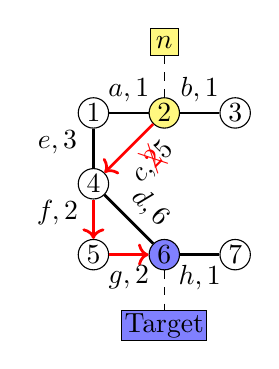
\begin{tikzpicture}
                \tikzset{Vertex/.style={%
                    shape=circle,%
                    draw=black,%
                    minimum size=10pt,%
                    radius=0.7cm,%
                    inner sep=1pt,%
                    node distance=0.9cm,%
                }}
                \tikzset{Note/.style={%
                    shape=rectangle,%
                    draw=black,%
                    minimum size=10pt,%
                    inner sep=1pt,%
                    node distance=0.9cm,%
                }}
            
                \node[Vertex] (1) {$1$};
                \node[Vertex, right of=1, fill=yellow!50] (2) {$2$};
                \node[Vertex, right of=2] (3) {$3$};
                \node[Vertex, below of=1] (4) {$4$};
                \node[Vertex, below of=4] (5) {$5$};
                \node[Vertex, right of=5, fill=blue!50] (6) {$6$};
                \node[Vertex, right of=6] (7) {$7$};

                \node[Note, above of=2, fill=yellow!50] (n) {$n$};
                \node[Note, below of=6, fill=blue!50] (target) {Target};

                \path (2) edge[-., dashed] (n);
                \path (6) edge[-., dashed] (target);
        
                \path (2) edge[-,line width=1pt] node[above]{\color{black}$a,1$} (1);
                \path (2) edge[-,line width=1pt] node[above]{\color{black}$b,1$} (3);
                \path (2) edge[->,line width=1pt, color=red] node[below,sloped,pos=0.4]{{\color{black} $c,$}{\color{red} \xcancel{2}}{\color{black}5}} (4);
                \path (4) edge[-,line width=1pt] node[above,sloped,pos=0.6]{\color{black}$d,6$} (6);
                \path (1) edge[-,line width=1pt] node[above,xshift=-13pt,yshift=-6pt]{\color{black}$e,3$} (4);
                \path (4) edge[->,line width=1pt, color=red] node[above,xshift=-13pt, yshift=-6pt]{\color{black}$f,2$} (5);
                \path (5) edge[->,line width=1pt, color=red] node[below]{\color{black}$g,2$} (6);
                \path (6) edge[-,line width=1pt] node[below]{\color{black}$h,1$} (7);
            \end{tikzpicture}
        \end{figure}
    \end{itemize}

\end{frame}

\begin{frame}{\CPDPathsName{} for early terminating the search}

    \textbf{Early search termination}: if the \CPDPath{$n$}{$t$} is not perturbated, then we already know an optimal path for going from $n$ to $t$ in the perturbated graph as well!
    \begin{minipage}{0.65\textwidth}

        \begin{center}
            if $\CPDPathCostNew{n}{t} = \CPDPathCostOriginal{n}{t}$
            
            $\downarrow$
            
            optimal solution is $\pathOnGraph{s}{n} \doublePlus{} \CPDPath{n}{t}$;

            \medskip

            $(s, t) = (2, 6)$
        
            $\CPDPathCostOriginal{4}{6} = 4$

            $\CPDPathCostNew{4}{6} = 4$
        \end{center}
    \end{minipage}\hfill%
    \begin{minipage}{0.35\textwidth}
        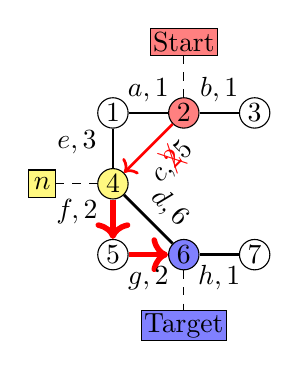
\begin{tikzpicture}
            \tikzset{Vertex/.style={%
                shape=circle,%
                draw=black,%
                minimum size=10pt,%
                radius=0.7cm,%
                inner sep=1pt,%
                node distance=0.9cm,%
            }}
            \tikzset{Note/.style={%
                shape=rectangle,%
                draw=black,%
                minimum size=10pt,%
                inner sep=1pt,%
                node distance=0.9cm,%
            }}
        
            \node[Vertex] (1) {$1$};
            \node[Vertex, right of=1, fill=red!50] (2) {$2$};
            \node[Vertex, right of=2] (3) {$3$};
            \node[Vertex, below of=1, fill=yellow!50] (4) {$4$};
            \node[Vertex, below of=4] (5) {$5$};
            \node[Vertex, right of=5, fill=blue!50] (6) {$6$};
            \node[Vertex, right of=6] (7) {$7$};

            \node[Note, above of=2, fill=red!50] (start) {Start};
            \node[Note, left of=4, fill=yellow!50] (n) {$n$};
            \node[Note, below of=6, fill=blue!50] (target) {Target};

            \path (2) edge[-., dashed] (start);
            \path (4) edge[-., dashed] (n);
            \path (6) edge[-., dashed] (target);
    
            \path (2) edge[-,line width=1pt] node[above]{\color{black}$a,1$} (1);
            \path (2) edge[-,line width=1pt] node[above]{\color{black}$b,1$} (3);
            \path (2) edge[->,line width=1pt, color=red] node[below,sloped,pos=0.4]{{\color{black} $c,$}{\color{red} \xcancel{2}}{\color{black}5}} (4);
            \path (4) edge[-,line width=1pt] node[above,sloped,pos=0.6]{\color{black}$d,6$} (6);
            \path (1) edge[-,line width=1pt] node[above,xshift=-13pt,yshift=-6pt]{\color{black}$e,3$} (4);
            \path (4) edge[->,line width=2pt, color=red] node[above,xshift=-13pt, yshift=-6pt]{\color{black}$f,2$} (5);
            \path (5) edge[->,line width=2pt, color=red] node[below]{\color{black}$g,2$} (6);
            \path (6) edge[-,line width=1pt] node[below]{\color{black}$h,1$} (7);
        \end{tikzpicture}
    \end{minipage}
\end{frame}

\begin{frame}{\CPDSearch{}}

    \begin{block}{\CPDSearch{}}
        \A{} variant yielding bounded suboptimal solutions where \CPDPathsName{} are exploited for searching the perturbated map (for brevity, we focus on the optimal working mode)
    \end{block}

    \begin{itemize}
        \item \CPDSearch{} maintains the best solution found and solution bounds (allows usage in anytime search);
        \item bounds computed thanks to $\CPDPathCostOriginal{n}{t}$ and $\CPDPathCostNew{n}{t}$;
        \item a threshold can be set to make the algorithm yields bounded suboptimal solutions (if the threshold is 1, the algorithm yields optimal solutions).
    \end{itemize}

\end{frame}

\begin{frame}{Experiment Results}
    \begin{itemize}
        \item Benchmark from moving AI [Sturtevant 2012];
        \item perturbation policy: along query optimal path we have generated a perturbated area (radius 15, costs increased up to factor of 4);
        \item comparison performed against ALT[Goldberg and Harrelson, 2005].
    \end{itemize}

    \begin{adjustwidth}{-2.5em}{-2.5em}
        \begin{minipage}{0.59\textwidth}
            \begin{figure}
                \centering
                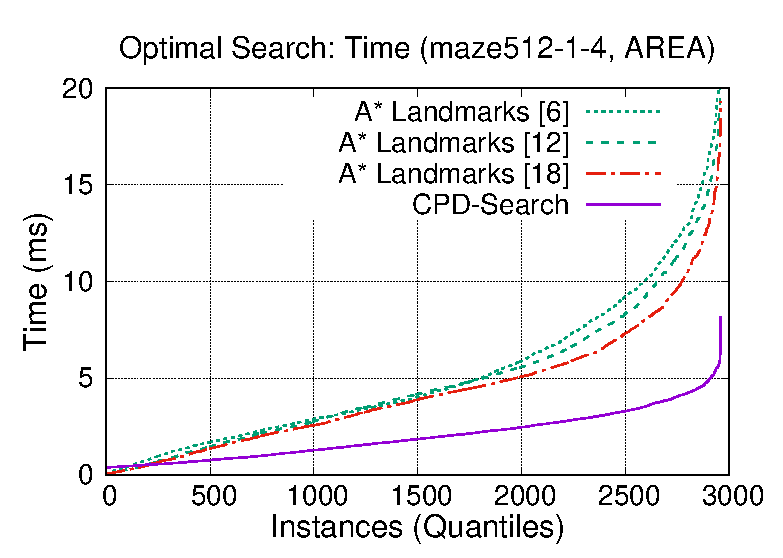
\includegraphics[width=1.0\textwidth]{src/images/pathfinding/optimal/maze512-1-4}
            \end{figure}
        \end{minipage}%
        \begin{minipage}{0.59\textwidth}
            \begin{figure}
                \centering
                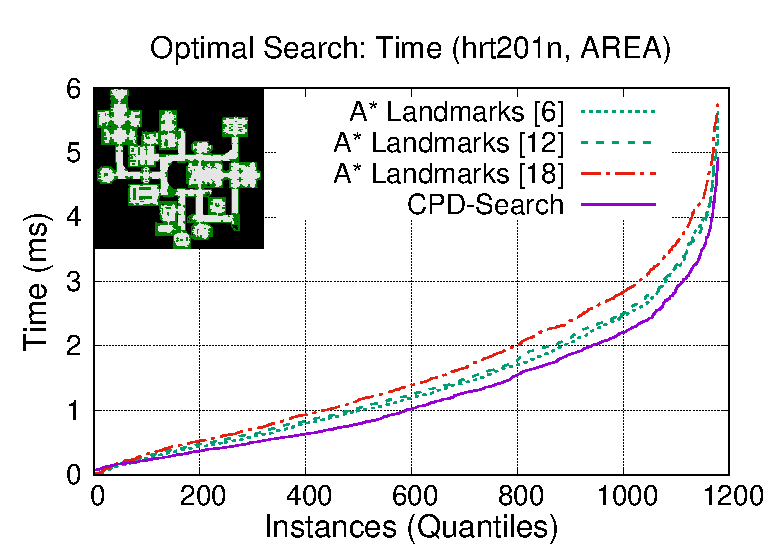
\includegraphics[width=1.0\textwidth]{src/images/pathfinding/optimal/hrt201n}
            \end{figure}
        \end{minipage}
    \end{adjustwidth}
\end{frame}
\section*{Conclusions}

\begin{frame}{Conclusions and Future Works}

    In the work we have:
    \begin{itemize}
        \item Investigated two new dynamic problems using graph-based knowledge;
        \item proposed algorithms efficiently solving the problem variants;
        \item the algorithms (\DPASATAlgorithmName{}, \DOHSATAlgorithmName{}, \CPDSearch{}) have been experimentally evaluated. The analysis shows significant gains \wrt{} \stateofart{};

        \item \textbf{Future works}: 
            The decremental consistency checking problem can be investigated in other algebra (\eg{} spatial); 
            or it can be use to find the minimal set of constraint relaxation making an inconsistent \TCSPName{} consistent;
            \CPDSearch{} can be (possibly) further improved by integrating a focal list to improve performance (\eg{} when the early termination mechanism is of little help).
    \end{itemize}
\end{frame}

\usebackgroundtemplate{%
	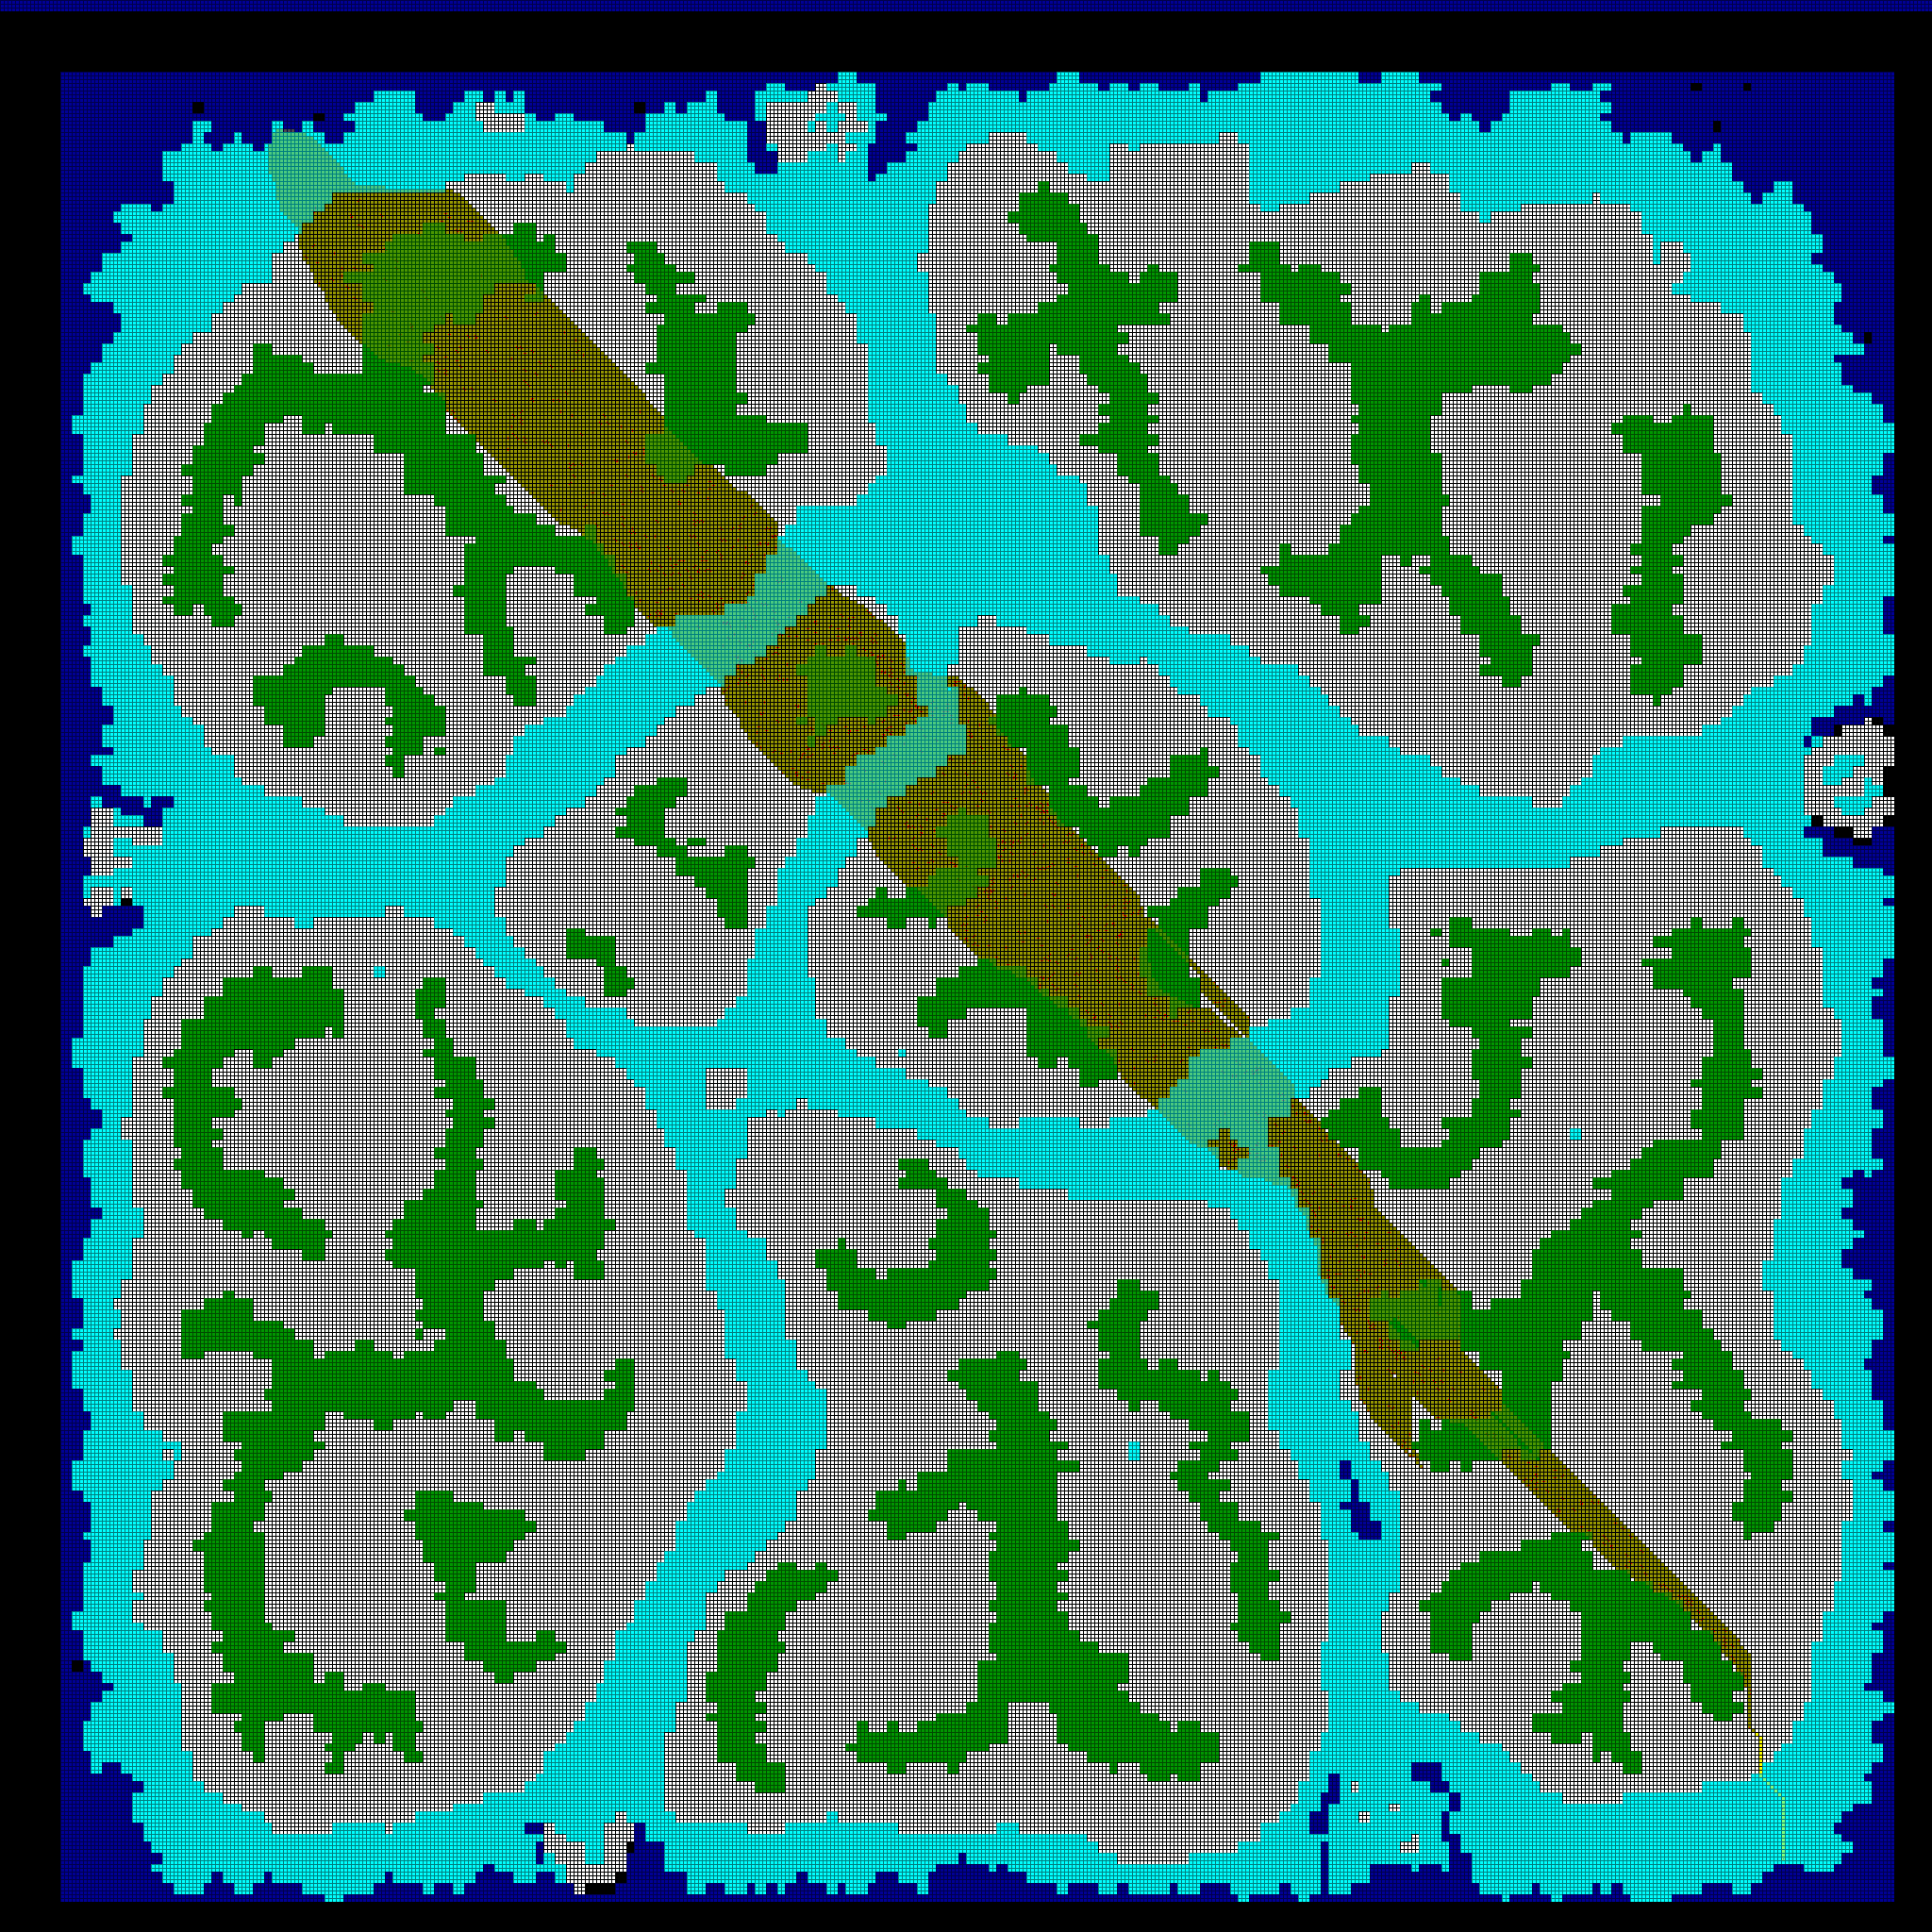
\includegraphics[width=\paperwidth,height=\paperheight]{src/images/pathfinding/cpdsearch}%
}
\begin{frame}[plain]
    \centering \Huge \textbf{Thanks for listening!\\Questions???}
\end{frame}


\end{document}
